\documentclass[pre,amssymb,showpacs,showkeys,preprint]{revtex4}
%\usepackage[T1]{fontenc}
\usepackage{bbm}
\usepackage{graphicx}
\usepackage{amsmath, amsthm, amssymb}
\newtheorem{prop}{Proposition}
\newtheorem{theorem}{Theorem}
\newtheorem{lemma}{Lemma}
\newtheorem{cor}{Corollary}

\usepackage{cdmtcs}
\begin{document}


\cdmtcsauthor{Martin Schaller and Karl Svozil}
\cdmtcstitle{Scale-Invariant Cellular Automata and Recursive Petri Nets}
\cdmtcsaffiliation{Vienna University of Technology}
\cdmtcstrnumber{347}
\cdmtcsdate{February 2009}
\colourcoverpage


\title{Scale-Invariant Cellular Automata and Recursive Petri Nets}

\author{Martin Schaller}
\email{martin_schaller@acm.org}
\affiliation{Algorithmics,
Parkring 10, 1010  Vienna, Austria}

\author{Karl Svozil}
\email{svozil@tuwien.ac.at}
\homepage{http://tph.tuwien.ac.at/~svozil}
\affiliation{Institut f\"ur Theoretische Physik, University of Technology Vienna,
Wiedner Hauptstra\ss e 8-10/136, A-1040 Vienna, Austria}




\begin{abstract}
Two novel computing models based on an infinite tesselation of space-time are introduced. They consist of recursively coupled primitive building blocks. The first model is a scale-invariant generalization of cellular automata, whereas the second one utilizes Petri net transitions. Both models are capable of hypercomputations and can, for instance, ``solve'' the halting problem for Turing machines. These two models are closely related, as they exhibit a step-by-step equivalence for finite computations. On the other hand, they differ greatly for infinite computations: the first one shows indeterministic behavior whereas the second one halts. Both models are capable of challenging our understanding of computability, causality, and space-time.
\end{abstract}


\pacs{05.90.+m,02.90.+p,47.54.-r}
\keywords{Cellular Automata, pattern formation}


\maketitle

\section{Introduction}
%Cellular automata are defined on a regular lattice.
%Mapping this lattice to Euclidean space introduces a natural unit of length, the distance
%between two adjacent cells.
%We extend the cellular automaton model by nesting an infinite number of lattices recursively.
%Choosing an appropriate timing behavior, we are able to achieve a constant speed of information
%propagation throughout the nested lattices.
%To our knowledge, this is the first computational model, which is scale invariant.
%We show that, due to the scale invariance and the constant information propagation speed, this new
%computational model has hypercomputing capabilities, i.e. is capable to solve Turing's Halting
%problem.

Every physically relevant computational model must be mapped into physical space-time and {\it vice versa}
\cite{landauer-89,maxwell-demon,bennett-73}.
In this line of thought, Von Neumann's self-reproducing Cellular Automata \cite{v-neumann-66}
have been envisioned by Zuse \cite{zuse-67,zuse-69,zuse-94,zuse-70}
and other researchers  \cite{fredkin,toffoli-margolus-90,wolfram-2002}
as  ``calculating space;''
i.e., as a
locally connected grid of finite automata \cite{hopcroft}
capable of universal algorithmic tasks, in which
intrinsic~\cite{svozil-94} observers are embedded~\cite{toffoli:79}.
This model is conceptually discreet and
noncontinuous and resolves the eleatic ``arrow''
antinomy \cite{zeno,ki-57,gruenbaum:68,sv-aut-rev}
against motion in discrete space by introducing
the concept of information about the state of motion in between time steps.

Alas,  there is no direct physical evidence supporting  the assumption of a tesselation of configuration space or time.
Given enough energy, and without the possible bound at the Planck length of about $10^{-35}$m, physical configuration space seems
to be potentially infinitely divisible.

Indeed, infinite divisibility of space-time has been utilized for proposals of a kind of ``Zeno oracle''~\cite{weyl:49},
a progressively accelerated Turing machine~\cite{gruenbaum:74,svozil98,rucker,Davies01,ord-2006}
capable of hypercomputation~\cite{Davis-2004,Doria-2006,Davis-2006}.
Such accelerated Turing machines have also been discussed in the relativistic context~\cite{thom:54,benna:62,pit:90,ear-nor:93,hogarth1,hogarth2,beth-59,le-91}.

The following models unify the conceptional clarity of
von Neumann's Cellular Automaton model with the
requirement of infinite divisibility of cell space.

\section{Scale-Invariant Cellular Automata}
\label{chap:sica}

\emph{Cellular automata} are dynamical systems in which space and time are discreet.
The states of cells in a regular lattice are updated synchronously according to a local deterministic
interaction rule.
The rule gives the new state of each cell as a function of the old states of some ``nearby'' states of its neighbor cells.
Each cell obeys the same rule, and has a finite (usually small) number of states.
For a more comprehensive introduction to cellular automata, we refer to Refs.~\cite{v-neumann-66,wolfram-86,gutowitz,ilachinski01,wolfram-2002}.

A \emph{scale-invariant cellular automaton} (SCA) operates like an ordinary
\emph{cellular automaton} (CA) on a cellular space, consisting of a regular arrangement of cells,
whereby each cell can hold a value from a set of discrete states.
Whereas the cellular space of a CA consists of a regular one- or higher
dimensional lattice, an SCA operates on a cellular space of recursively nested lattices
which can be embedded in some Euclidean space as well.

The time behavior of an SCA differs from the time behavior of CA:
Cells in the same lattice synchronously change their state \cite{Morelli_Zanette}, but
as cells are getting smaller in deeper nested lattices, the time steps between state changes in
the same lattice are assumed to {\em decrease} and approach zero in the limit.
Thereby, a finite speed of signal propagation between adjacent cells is always maintained.
The SCA model gains its  computing capabilities by introducing a local rule that
allows for interaction between adjacent lattices \cite{BoFeng_MengDing}.
We will introduce the SCA model for the one-dimensional case, the extension to higher dimensions
\cite{Brunnet_Chate} is
straightforward.

An SCA, like a CA, is defined by a cellular space, a topology that defines the neighborhood of a cell, a finite set of
states a cell can be in,  a time model that determines when a cell is updated, and a local rule that
maps states of neighborhood cells to a state.
We first define the cellular space of an SCA.
To this end, we make use of the standard interval arithmetic.
For a scalar $\lambda \in \mathbb{R}$ and a (half-open) interval $[x,y) \subset \mathbb{R}$ set:
$\lambda + [x,y) = [\lambda + x, \lambda + y)$ and $\lambda [x,y) = [\lambda x, \lambda y)$.
We denote the unit interval $[0,1)$ by $\mathbbm{1}$.
Let $L_k$ be the lattice that partitions the real numbers in half-open intervals of length $2^k$, where $k$ is an integer:
$L_k = \{2^k (i + \mathbbm{1})| i \in \mathbb Z\}$.
 The cellular space $\mathcal{C}$, the set of all cells of the SCA, is the union of all lattices $L_k$:
$\mathcal{C} = \bigcup_{k \in \mathbb Z} L_k = \{ 2^k (i + \mathbbm{1}) | i, k \in \mathbb Z\}$.

\begin{figure}
\begin{center}
\scalebox{0.7}{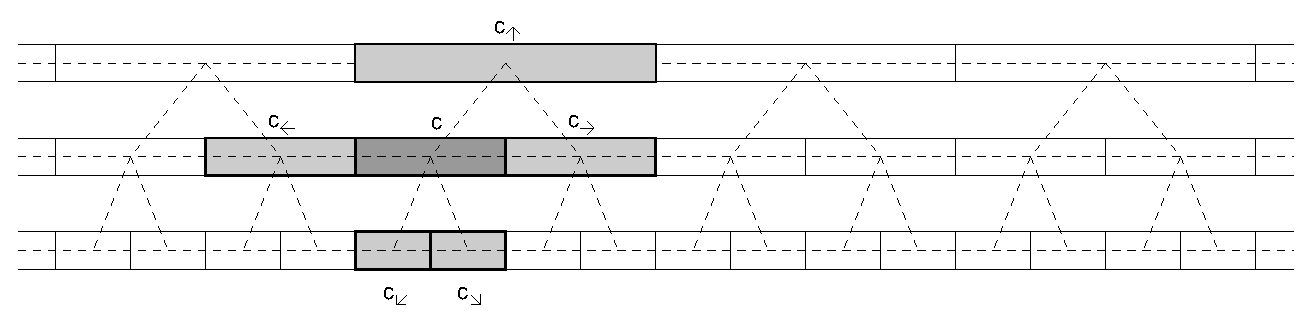
\includegraphics{2008-sica-spaceoperators.eps}}
\caption{\label{fig:1-dim-interaction} Space and topological structure of an SCA.}
\end{center}
\end{figure}

Next, we define the neighborhood of a cell by a set of operators $\mathit{op}: \mathcal{C} \rightarrow \mathcal{C}$.
For a cell $c = 2^k (i + \mathbbm{1})$ in $\mathcal{C}$ let
$c_{\leftarrow} = 2^k (i - 1 + \mathbbm{1})$ be the left neighbor,
$c_{\rightarrow} = 2^k (i + 1 + \mathbbm{1})$ the right neighbor,
$c_{\uparrow} =  2^{k + 1} (\lfloor \frac{i}{2} \rfloor + \mathbbm{1})$ the parent,
$c_{\swarrow} = 2^{k-1}(2i + \mathbbm{1})$ the left child,
and $c_{\searrow} = 2^{k-1}(2i + 1 + \mathbbm{1})$ the right child of $c$.
This topology is depicted in Fig.~\ref{fig:1-dim-interaction}.
The predicate $\mathit{left}(c)$ is true if and only if the cell $c$ is the left child of its parent.
Analogously, $\mathit{right}(c)$ is true if and only if the cell $c$ is the right child of its parent.
Obviously, for all cells $c$ either $\mathit{left}(c)$ or $\mathit{right}(c)$ is true.

\begin{figure}
\begin{center}
\scalebox{0.7}{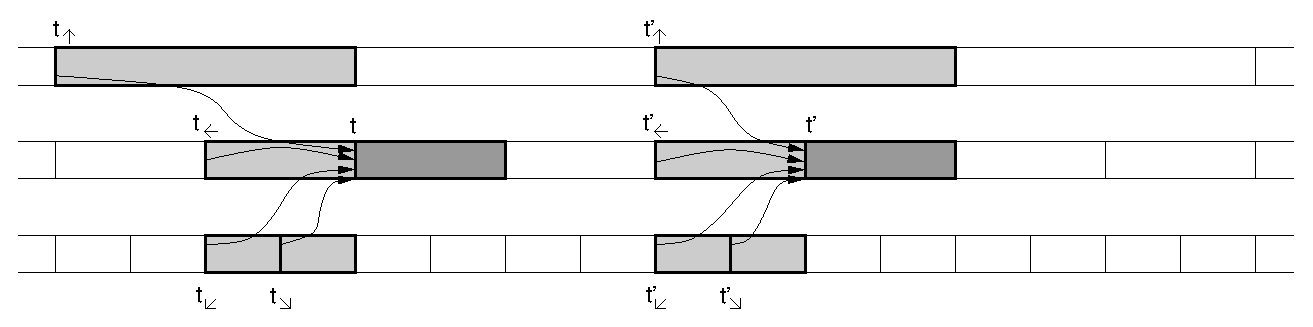
\includegraphics{2008-sica-timeoperators.eps}}
\caption{\label{fig:timeops} Temporal dependencies of an SCA.}
\end{center}
\end{figure}

All cells in lattice $L_k$ are updated synchronously at time instances $2^k i$ where $i$ is an integer.
The time interval between two cell updates in lattice $L_k$ is again a half-open interval $2^k (i + \mathbbm{1})$
and the cycle time, that is the time between two updates of the cell, is therefore $2^k$.
A simple consequence of this time model is that child cells cycle twice as fast and the parent cell cycle
half as fast as the cell itself.
The time space $\mathcal{T}$ is the set of all possible time intervals, which is in the one-dimensional
case equal to the set $\mathcal{C}$: $\mathcal{T} = \{ 2^k (i + \mathbbm{1}) | i, k \in \mathbb Z\}$.

Analogously to the neighborhood operators of the cellular space we define temporal operators which express
the temporal dependencies of a cell update.
The usage of time intervals instead of time instances, has the advantage
that a time interval uniquely identifies the lattice where the update occurs.
Each time operator is a mapping $\mathit{op}: \mathcal{T} \rightarrow \mathcal{T}$.
For a time inverval $t = 2^k (i + \mathbbm{1})$ let
$t_\leftarrow = 2^k (i - 1 + \mathbbm{1})$,
$t_\uparrow = 2^{k + 1} (\lfloor \frac{i-1}{2} \rfloor + \mathbbm{1})$,
$t_\swarrow = 2^{k-1} (2i - 2  + \mathbbm{1})$, and
$t_\searrow =  2^{k-1} (2i - 1 + \mathbbm{1})$.
These time operators express the temporal dependencies of a cell update.
The predicate $\mathit{sync}(t)$ is true if and only if $i$ is even.
If $\mathit{sync}(t)$ is true, the state change of a cell in $L_k$ at the beginning of $t$ occurs
synchronous with the state change of its parent cell, otherwise asynchronous,
which is expressed by the predicate $\mathit{async}(t) = \neg \mathit{sync}(t)$.
Fig.~\ref{fig:timeops} depicts the temporal dependencies of a cell: to the left it shows a
synchronous state change, to the right an asynchronous one.
We remark that we denoted space and time operators by the same symbols, even if their mapping is different.
In applying these operators, we take in the remainder of this paper care, that the context of the operator is always clearly defined.

At any time, each cell is in one state from a finite state set $Z$.
The cell state in a given time interval is described by the state function $s(c,t)$,
which maps cells and time intervals to the state set.
The space-time $\mathcal{S}$ of the SCA describes the combinations of allowed combinations of cells and time intervals:
$\mathcal{S} = \{(c,t)| c \in \mathcal{C}, t \in \mathcal{T} \mbox{ and } |c| =|t|\}$.
Then, the state function $s$ can be expressed as a mapping $s: \mathcal{S} \rightarrow Z$.
The local rule describes the evolution of the state function.
It consists of four functions, whereby for a given cell and time interval only one
function is applicable, depending whether the cell is the left or the right child of its parent cell and
whether the state change is synchronous or asynchronous to the state change of its parent cell.
For a cell $c$ and a time interval $t$, where $(c, t)$ is in $\mathcal{S}$, the
evolution of the state is given by the local rule of the SCA
\begin{equation}
\label{eq:local-rule}
\footnotesize
s(c,t) = \left\{
\begin{array}{l}
f_{LA}(
        s(c_\uparrow, t_\uparrow),
        s(c_\leftarrow, t_\leftarrow), s(c, t_\leftarrow), s(c_\rightarrow, t_\leftarrow),
        s(c_\swarrow, t_\swarrow), s(c_\searrow, t_\swarrow),
        s(c_\swarrow, t_\searrow), s(c_\searrow, t_\searrow)
)
\\
\hspace{0.3in} \mbox{ if  $\mathit{left}(c)$ and $\mathit{async}(t)$;} \vspace{0.1in}
\\
f_{LS}(
        s(c_\uparrow, t_\uparrow),
        s(c_\leftarrow, t_\leftarrow), s(c, t_\leftarrow), s(c_\rightarrow, t_\leftarrow),
        s(c_\swarrow, t_\swarrow), s(c_\searrow, t_\swarrow),
        s(c_\swarrow, t_\searrow), s(c_\searrow, t_\searrow)
)
\\
\hspace{0.3in} \mbox{if $\mathit{left}(c)$ and $\mathit{sync}(t);$}  \vspace{0.1in}
\\
f_{RA}(
        s(c_\uparrow, t_\uparrow),
        s(c_\leftarrow, t_\leftarrow), s(c, t_\leftarrow), s(c_\rightarrow, t_\leftarrow),
        s(c_\swarrow, t_\swarrow), s(c_\searrow, t_\swarrow),
        s(c_\swarrow, t_\searrow), s(c_\searrow, t_\searrow)
)
\\
\hspace{0.3in} \mbox{if $\mathit{right}(c)$ and $\mathit{async}(t)$;} \vspace{0.1in}
\\
f_{RS}(
        s(c_\uparrow, t_\uparrow),
        s(c_\leftarrow, t_\leftarrow), s(c, t_\leftarrow), s(c_\rightarrow, t_\leftarrow),
        s(c_\swarrow, t_\swarrow), s(c_\searrow, t_\swarrow),
        s(c_\swarrow, t_\searrow), s(c_\searrow, t_\searrow)
)
\\
\hspace{0.3in} \mbox{if $\mathit{right}(c)$ and $\mathit{sync}(t).$} \\

\end{array}
\right.
\end{equation}
Formally, an SCA $A$ is denoted by the tuple $A = (Z, f_{LA}, f_{LS}, f_{RA}, f_{RS})$.
We remark that the application of the local rule in its general form might lead to indeterministic behaviour.
We will give an analysis of this phenomenon and a resolution later on.
A special case of the local rule is a rule of the form
$f(s(c_\leftarrow, t_\leftarrow), s(c, t_\leftarrow), s(c_\rightarrow, t_\leftarrow))$,
which is the constituting rule of a one-dimensional 3-neighborhood CA.
In this case, the SCA splits up in a sequence of infinitly many nonconnected CAs.
This shows that the SCA model is truly an extension of the CA model and allows us to
view an SCA as an infinite sequence of interconnected CAs.

We now examine the signal speed that is required to communicate state changes between neighbor cells.
To this end, we select the middle point of a cell as the source and the target of a
signal that propagates the state change of a cell to one of its neighbor cells.
A simple consideration shows that the most restricting cases are the paths from the space time points
$(c_\leftarrow, t_\leftarrow)$, $(c_\uparrow, t_\uparrow)$, $(c_\swarrow, t_\searrow)$ to $(c,t)$ for $\mathit{async}(t)$.
The simple calculation delivers the results $1,1$, and $\frac{1}{2}$, respectively,
hence a signal speed of 1 is sufficient to deliver the updates in the given timeframe.
A more general examination takes also the processing time of a cell into account.
If a cell in $L_k$ takes time $2^k p$ and we assume a finite signal speed of $v$,
the cycle time of a cell in $L_k$ must be at least $2^k (p + v)$.
In sum, as long as the processing time is proportional to the diameter of a cell,
we can always find a scaling factor $t \rightarrow \lambda t$, such that
the SCA has cycle times that conform to the time space $\mathcal{T}$.

The construction of a hypercomputer in section \ref{chap:hypercomputer} makes use of a simplified version of an SCA, which we call
a Recursive Cellular Automaton (RCA).
The cellular space of a RCA is the set $\mathcal{C} = \{2^k \mathbbm{1} | k \in \mathbb Z\}$.
The time space $\mathcal{T}$ of a RCA is the same as for an SCA: $\mathcal{T} = \{2^k (i + \mathbbm{1})| i, k \in \mathbb{Z}\}$.
The neighborhood operators $c_\uparrow$ and $c_\swarrow$ can still be applied as well as all time operators.
The state set $Z$ is again a finite set.
The space-time of a RCA is the set $\mathcal{S} = \{(c,t)| c \in \mathcal{C}, t \in \mathcal{T} \mbox{ and } |c| = |t|\}$.
The RCA has the following local rule: for all $(c, t) \in \mathcal{S}$
\begin{equation}
s(c,t) = \left\{
\begin{array}{l}
f_{A}(
        s(c_\uparrow, t_\uparrow),
        s(c, t_\leftarrow),
        s(c_\swarrow, t_\swarrow),
        s(c_\swarrow, t_\searrow)
) \mbox{  if $\mathit{async}(t)$;} \\
f_{S}(
        s(c_\uparrow, t_\uparrow),
        s(c, t_\leftarrow),
        s(c_\swarrow, t_\swarrow)
        s(c_\swarrow, t_\searrow)
) \mbox{  if $\mathit{sync}(t)$.} \\
\end{array}
\right.
\end{equation}
Formally, a RCA $A$ is denoted by a tuple $A = (Z, f_A, f_S)$.
By restricting the local rule of an SCA, a RCA can also be constructed from an SCA.
Consider an SCA, whose local rule does not depend on
the cell neighbors $c_\leftarrow$, $c_\rightarrow$, and $c_\searrow$.
Then, the resulting SCA contains the RCA as subautomaton.

For convenience we introduce the following notation for RCAs.
We index a cell $[0, 2^k)$ by the integer $-k$, that is a cell with index $k$ has a cyle time of $2^{-k}$.
We call the cell $k - 1$ the upper neighbor and the cell $k + 1$ the lower neighbor of cell $k$.
Time instances can be conveniently expressed as a binary number.
If not other said, we use the cycle time of cell 0 as time unit.

We noted before that the evolution of an SCA might lead to indeterministic behavior.
This holds also for RCAs, which we will use to analyze this phenomenon.
Consider an initial configuration of a RCA at time 0.
That is, the state of a cell $k$ is defined for the half-open time interval $[0, 2^{-k})$.
We want to calculate the state of cell 0 at time 1.
To apply the local rule on cell 0 we have to know the state of cell 1 at time $0.1_2$.
The state of cell 1 at time $0.1_2$ depends on the state of cell 2 at time $0.01_2$.
In general the state of cell $i$ at time $2^{-i}$ depends on the state of cell $i + 1$ at time $2^{-(i+1)}$.
This is an infinite regress that leads us to the conclusion that in the general case the state of cell 0 at time $1$ does not
depend on the initial configuration and therefore the state of a cell $k$ at time $2^{-k}$ is indeterministic.
A similar paradox arises, if the state change of cell $i$ at time $t$ depends on the state of cell $i + 1$ at time
$t_\swarrow$, but does not dependent on the state at time $t_\searrow$.
The first evolution of cell $0$ will be deterministic, but the next time step would again lead to an indeterministic value of cell $0$.
We will come back to this problem and view it from a different perspective in section \ref{chap:petri}.
For now, we offer the following two solutions to this problem, both based on a quiescent state $q$.

\begin{enumerate}

\item \emph{(Short-circuit evaluation)}
Let $q$ in $Z$ be the quiescent state with the following semantics.
Whenever a cell is in state $q$, the cell does not evaluate its lower neighbor.
The cell remains as long in the quiescent state as long as the upper neighbor is in the quiescent state, too,
that is $f_A(q, q, ?, ?) = f_S(q, q, ?, ?) = q$, where the question mark $?$ represents an arbitrary state.
This modus of operandi corresponds to the short-circuit evaluation of logical expressions in programming
languages like C or Java.
If the RCA starts now with an initial configuration of the form $z_0 z_1 \ldots z_n q q q\ldots$, starting at cell $0$, the infinite
regress is interrupted, since cell $n+2$ evaluates to $q$ without being dependent on cell $n+3$.

\item \emph{(Dynamically growing RCA)}
The second alternative consists of a RCA that starts initially with the finite set of cells $0, \ldots, n$ and the following
boundary condition.
Whenever cell $0$ or the cell with the highest index $k$ is evaluated, the state of the missing neighbor cell is assumed to be $q$.
The RCA dynamically appends cells to the lower end when needed:
whenever the cell with the highest index $k$ enters a state that is different from the quiescent state,
a new cell $k + 1$ is appended, initialized with state $q$, and connected to the cell $k$.
To be more specific: If $k$ is the highest index, and cell $k$ evaluates at time $2^{-k} i$ to state $z \neq q$,
a new cell $k + 1$ in state $q$ is appended.
The cell performs its first transition at time $2^{-k} (i + \frac{1}{2})$, assuming state $q$ for its missing lower neighbor cell.
We note that the same technique could also be applied to append upper cells to the RCA, although in the remainder of this paper, we deal only
with RCAs that are growing to the bottom.

\end{enumerate}

Both enhancements ensure a deterministic evaluation either for a configuration where only a finite number of cells is in a nonquiescent state
or for a finite number of cells.

\section{Constructing a Hypercomputer}
\label{chap:hypercomputer}
In this section, we construct an accelerated Turing machine from a RCA.
The RCA will simultaneously simulate the Turing machine and shift the tape content down
to faster cycling cells.

We use the following model of a Turing machine (TM) \cite{hopcroft}.
Formally, a Turing machine is a tuple
$M = (Q, \Sigma, \Gamma, \delta, q_0, B, F)$,
where $Q$ is the finite set of states, $\Gamma$ is the finite set of tape symbols,
$\Sigma \subset \Gamma$ is the set of input symbols, $q_0 \in Q$ is the start state,
$B \in \Gamma \backslash \Sigma$ is the blank, and $F \subset Q$ is the set of final states.
The next move function or transition function $\delta$ is a mapping from
$Q \times \Gamma$ to $Q \times \Gamma \times \{L, R\}$, which may be undefined for some arguments.
The TM $M$ works on a tape divided into cells that has a leftmost cell but is infinite to the right.
Let $\delta(q, a) = (p, b, D)$.
One step (or move) of $M$ in state $q$ and the head of $M$ positioned over input symbol $a$
consists of the following actions:
scanning input symbol $a$, replacing symbol $a$ by $b$,
entering state $p$ and moving the head one cell either to the left ($D=L$) or to the right ($D=R$).
In the beginning $M$ starts in state $q_0$ with a tape that is initialized with an input word $w \in \Sigma^*$,
starting at the leftmost cell, all other cells blank,
and the head of $M$ positioned over the first symbol of $w$.
We need sometimes the function $\delta$ split up into three separate functions:
$\delta(q,a) = (\delta_Q(q,a), \delta_\Gamma(q,a), \delta_D(q,a))$.

The configuration of a TM $M$ is denoted by an instantaneous description (ID) of the form
$\alpha_1 q \alpha_2$, where $q \in Q$ and $\alpha_1, \alpha_2 \in \Gamma^*$.
Here $q$ is the current state of $M$, $\alpha_1$ is the tape content to the left,
and $\alpha_2$ the tape content to the right of the head including the symbol that is scanned next.
Leading and trailing blanks will be omitted, except the head has moved to the left or to the right of
the non-blank content.

Let $\alpha_1 q \alpha_2$ and  $\alpha_1^\prime p \alpha_2^\prime$ be two IDs of $M$.
The relation $\alpha_1 q \alpha_2 \vdash_M \alpha_1^\prime p \alpha_2^\prime$ states
that $M$ with ID $\alpha_1 q \alpha_2$ changes in one step
to ID $\alpha_1^\prime p \alpha_2^\prime$.
The relation $\vdash_M^*$ denotes the reflexive and transitive closure of $\vdash_M$.

Let $M = (Q, \Sigma, \Gamma, \delta, q_0, B, F)$ be an arbitrary Turing machine.
We construct a RCA $A_M = (Z, f_S, f_A)$ that simulates $M$ as follows.
First, we do not need the dependency $t_\swarrow$, therefore we simplify the local rule to
\begin{equation}
s(c,t) = \left\{
\begin{array}{l}
f_{a}(
        s(c_\uparrow, t_\uparrow),
        s(c, t_\leftarrow),
        s(c_\swarrow, t_\searrow)
) \mbox{  if $\mathit{async}(t)$;} \\
f_{s}(
        s(c_\uparrow, t_\uparrow),
        s(c, t_\leftarrow),
        s(c_\swarrow, t_\searrow)
) \mbox{  if $\mathit{sync}(t)$.} \\
\end{array}
\right.
\end{equation}
The state set $Z$ is given by
\[
Z = \Gamma \cup (\Gamma \times \{\rightarrow\}) \cup (Q \times \Gamma)
\cup (Q \times \Gamma \times \{\rightarrow\}) \cup
\{\Box, \blacktriangleleft, \lhd, \vec{\lhd}, \rhd, \rhd_B, \rhd_\blacktriangleleft\}.
\]
We write $\overrightarrow{a}$ for an element $(a, \rightarrow)$ in $\Gamma \times \{\rightarrow\}$
and $\overrightarrow{\langle q,a \rangle}$ for an element
$\langle q, a, \rightarrow \rangle$ in $Q \times \Gamma \times \{\rightarrow\}$.
To simulate $M$ on the input $w=a_1 \ldots a_n$ in $\Sigma^*$, $n \geq 1$,
$A_M$ is initialized with the sequence
$\overrightarrow{\lhd} \langle q_0,a_1 \rangle a_2 a_3\ldots a_n\rhd $
starting at cell 0, all other cells shall be in the quiescent state $\Box$.
If $w=a_1$, $A_M$ is initialized with the sequence
$\overrightarrow{\lhd} \langle q_0,a_1 \rangle B\rhd $, and
if $w=\epsilon$, the empty word, $A_M$ is initialized with the sequence
$\overrightarrow{\lhd} \langle q_0,B \rangle B\rhd $.
We denote the initial configuration by $C_0$, or by $C_0(w)$ if we want to emphasize the dependency on the input word $w$.
The computation is started at time 0, i.e. the first state change of cell $k$ occurs at time $2^{-k}$.

The elements $\langle q, a \rangle$ and $\overrightarrow{\langle q, a \rangle}$  act as head of the
Turing Machine including the input symbol of the Turing Machine that is scanned next.
To accelerate the TM, we have to shift down the tape content to faster cycling cells of the RCA,
thereby taking care that the symbols that represent the non-blank content of the TM tape are kept together.
We achieve this by sending a pulse from the left delimiter $\lhd$ to the right delimiter $\rhd$ and back.
Each zigzag of the pulse moves the tape content one cell downwards and triggers
at least one move of the TM.
Furthermore a blank is inserted to the right of the simulated head if necessary.
The pulse that goes down is represented by exactly one element of the form
$\overrightarrow{\lhd}, \overrightarrow{a}, \overrightarrow{\langle q,a \rangle}, \rhd_B$, or $\rhd_\blacktriangleleft$,
the upgoing pulse is represented by the element $\blacktriangleleft$.

The specification of the values for the functions $f_A$ and $f_S$ for all possible triples of
cell states is tedious, therefore we use the following approach.
A synchronous transition of two neighbor cells can perform a simultaneous state change of the two cells.
If the state change of these two neighbor cells is independent of their other neighbors,
we can specify the state change as a transformation of a state pair into another one.
Let $z_1, z_2, z_1^\prime, z_2^\prime$ be elements in $Z$.
The block transformation $z_1 \: z_2 \mapsto z_1^\prime \: z_2^\prime$ defines
 a function mapping of the form
$
f_A(x, z_1, z_2) = f_S(x, z_1, z_2) = z_1^\prime
$
and
$
f_S(z_1, z_2,y) = z_2^\prime
$
for all $x, y$ in $Z$.
Furthermore, we will also allow block transformations that might be ambigious for certain configurations.
Consider the block transformations
$z_1 \: z_2 \mapsto z_1^\prime \: z_2^\prime$
and
$z_2 \: z_3 \mapsto z_2^{\prime\prime} \: z_3^\prime$
that might lead to an ambiguity for a configuration that contains $z_1z_2z_3$.
Instead of resolving these ambiguities in a formal way, we will restrict our consideration to
configurations that are unambiguous.

The evolution of the RCA $A_M$ is governed by the following block transformations:
\begin{enumerate}

\item
\emph{Pulse moves downwards.}
Set
\begin{equation}
\overrightarrow{\lhd} \: \langle q, a \rangle \mapsto \lhd \:
\overrightarrow{\langle q, a \rangle};
\label{tr:start-state}
\end{equation}
\begin{equation}
\overrightarrow{a} \: b \mapsto a \: \overrightarrow{b};
\label{tr:down}
\end{equation}
\begin{equation}
\overrightarrow{\lhd} \:a \mapsto \lhd \: \overrightarrow{a}.
\label{tr:start}
\end{equation}
If $\delta(q,a) = (p,c,R)$ set
\begin{equation}
\overrightarrow{b} \: \langle q, a \rangle \mapsto b \:
\overrightarrow{\langle q, a \rangle};
\label{tr:down-to-head}
\end{equation}
\begin{equation}
\overrightarrow{\langle q,a \rangle} \: b \mapsto c \:
\overrightarrow{\langle p, b \rangle};
\label{tr:right-2}
\end{equation}
\begin{equation}
\overrightarrow{\langle q,a \rangle} \: \rhd \mapsto \langle q,a \rangle \:
\rhd_B.
\label{tr:down-state-right-delimiter-blank}
\end{equation}
If $\delta(q,a) = (p,c,L)$ set
\begin{equation}
\overrightarrow{b} \: \langle q, a \rangle \mapsto \langle p, b \rangle \:
\overrightarrow{c};
\label{tr:left-1}
\end{equation}
\begin{equation}
\overrightarrow{\langle q,a \rangle} \: b \mapsto \langle q,a \rangle \:
\overrightarrow{b};
\label{tr:left-no-move}
\end{equation}
\begin{equation}
\overrightarrow{\langle q,a \rangle} \: \rhd \mapsto \langle q,a \rangle \:
\rhd_\blacktriangleleft.
\label{tr:down-state-right-delimiter}
\end{equation}
Set
\begin{equation}
\overrightarrow{a} \: \rhd \mapsto a \: \rhd_\blacktriangleleft;
\label{tr:down-a-rhd}
\end{equation}
\begin{equation}
\rhd_B \: \Box \mapsto B \: \rhd_\blacktriangleleft;
\label{tr:new-blank}
\end{equation}
\begin{equation}
\rhd_\blacktriangleleft \: \Box \mapsto \blacktriangleleft \: \rhd.
\label{tr:reflection-right}
\end{equation}

\item
\emph{Pulse moves upwards}.
Set
\begin{equation}
a \: \blacktriangleleft \mapsto \blacktriangleleft \: a;
\label{tr:up}
\end{equation}
\begin{equation}
\langle q,a \rangle \: \blacktriangleleft \mapsto  \blacktriangleleft \:
\langle q,a \rangle;
\label{tr:up-state}
\end{equation}
\begin{equation}
\lhd \: \blacktriangleleft \mapsto \Box \: \overrightarrow{\lhd}.
\label{tr:up-lhd}
\end{equation}
\end{enumerate}

If to a certain cell no block transformation is applicable the cell shall remain in its previous state.
Furthermore, we assume a short-circuit evaluation with regard to the quiescent state:
$f_A(\Box, \Box, ?) = f_S(\Box, \Box, ?) = \Box$, whereby the lower neighbor cell is not evaluated.

\begin{figure}
\begin{center}
\renewcommand{\arraystretch}{0.7}
\begin{tabular}{c|ccccc}
& \multicolumn{5}{c}{ Symbol} \\
State & 0 & 1 & $X$ & $Y$ & $B$ \\ \hline
$q_0$ & $(q_1,X,R)$ & ---         & ---         & $(q_3,Y,R)$ & ---         \\
$q_1$ & $(q_1,0,R)$ & $(q_2,Y,L)$ & ---         & $(q_1,Y,R)$ & ---         \\
$q_2$ & $(q_2,0,L)$ & ---         & $(q_0,X,R)$ & $(q_2,Y,L)$ & ---         \\
$q_3$ & ---         & ---         & ---         & $(q_3,Y,R)$ & $(q_4,B,R)$ \\
$q_4$ & ---         & ---         & ---         & ---         & ---         \\
\end{tabular}
\end{center}
\caption{\label{fig:example-delta}The function $\delta$.}
\end{figure}

We illustrate the working of $A_M$ by a simple example.
Let $L$ be the formal language consisting of strings with $n$ 0's, followed by $n$ 1's:
$L = \{0^n1^n | n \geq 1\}$.
A TM that accepts this language is given by
$M = (\{q_0, q_1, q_2, q_3, q_4\}, \{0,1\}, \{0,1,X,Y,B\}, \delta, q_0, B, \{q_4\})$ \cite{hopcroft}
with the transition function depicted in Fig.~\ref{fig:example-delta}.
The computation of $M$ on input $01$ is given below:
\[
q_001 \vdash Xq_11  \vdash  q_2XY  \vdash  Xq_0Y  \vdash  XYq_3  \vdash XYBq_4.
\]
Fig.~\ref{fig:example-hyper-sca-2} depicts the computation of $A_M$ on the TM input 01.
The first column of the table specifies the time in binary base.
$A_M$ performs 4 complete pulse zigzags and enters a final configuration in the $5^{th}$ one after the TM simulation has reached
the final state $q_4$.
Fig.~\ref{fig:evolution} depicts the space-time diagram of the computation.
It shows the position of the left and right delimiter (gray) and the position of the pulse (black).

\begin{figure}
\begin{center}
\scriptsize     {
\renewcommand{\arraystretch}{0.9}
\begin{tabular}{r|cccccccccccccc}
   &0 &1 & 2 & 3 & 4 & 5 & 6 & 7 & 8 & 9 \\ \hline
$0.00000000_2$ & $\overrightarrow{\lhd}$ & $\langle q_0,0 \rangle$ & $1$ & $\rhd$ & $\Box$ & $\Box$ & $\Box$ & $\Box$ & $\Box$ & $\Box$ \\
$1.00000000_2$ & $\lhd$ & $\overrightarrow{\langle q_0,0 \rangle}$ & $1$ & $\rhd$ & $\Box$ & $\Box$ & $\Box$ & $\Box$ & $\Box$ & $\Box$ \\
$1.10000000_2$ & $\lhd$ & $X$ & $\overrightarrow{\langle q_1,1 \rangle}$ & $\rhd$ & $\Box$ & $\Box$ & $\Box$ & $\Box$ & $\Box$ & $\Box$ \\
$1.11000000_2$ & $\lhd$ & $X$ & $\langle q_1,1 \rangle$ & $\rhd_\blacktriangleleft$ & $\Box$ & $\Box$ & $\Box$ & $\Box$ & $\Box$ & $\Box$ \\
$1.11100000_2$ & $\lhd$ & $X$ & $\langle q_1,1 \rangle$ & $\blacktriangleleft$ & $\rhd$ & $\Box$ & $\Box$ & $\Box$ & $\Box$ & $\Box$ \\
$10.00000000_2$ & $\lhd$ & $X$ & $\blacktriangleleft$ & $\langle q_1,1 \rangle$ & $\rhd$ & $\Box$ & $\Box$ & $\Box$ & $\Box$ & $\Box$ \\
$10.10000000_2$ & $\lhd$ & $\blacktriangleleft$ & $X$ & $\langle q_1,1 \rangle$ & $\rhd$ & $\Box$ & $\Box$ & $\Box$ & $\Box$ & $\Box$ \\
$11.00000000_2$ & $\Box$ & $\overrightarrow{\lhd}$ & $X$ & $\langle q_1,1 \rangle$ & $\rhd$ & $\Box$ & $\Box$ & $\Box$ & $\Box$ & $\Box$ \\
$11.10000000_2$ & $\Box$ & $\lhd$ & $\overrightarrow{X}$ & $\langle q_1,1 \rangle$ & $\rhd$ & $\Box$ & $\Box$ & $\Box$ & $\Box$ & $\Box$ \\
$11.11000000_2$ & $\Box$ & $\lhd$ & $\langle q_2,X \rangle$ & $\overrightarrow{Y}$ & $\rhd$ & $\Box$ & $\Box$ & $\Box$ & $\Box$ & $\Box$ \\
$11.11100000_2$ & $\Box$ & $\lhd$ & $\langle q_2,X \rangle$ & $Y$ & $\rhd_\blacktriangleleft$ & $\Box$ & $\Box$ & $\Box$ & $\Box$ & $\Box$ \\
$11.11110000_2$ & $\Box$ & $\lhd$ & $\langle q_2,X \rangle$ & $Y$ & $\blacktriangleleft$ & $\rhd$ & $\Box$ & $\Box$ & $\Box$ & $\Box$ \\
$100.00000000_2$ & $\Box$ & $\lhd$ & $\langle q_2,X \rangle$ & $\blacktriangleleft$ & $Y$ & $\rhd$ & $\Box$ & $\Box$ & $\Box$ & $\Box$ \\
$100.01000000_2$ & $\Box$ & $\lhd$ & $\blacktriangleleft$ & $\langle q_2,X \rangle$ & $Y$ & $\rhd$ & $\Box$ & $\Box$ & $\Box$ & $\Box$ \\
$100.10000000_2$ & $\Box$ & $\Box$ & $\overrightarrow{\lhd}$ & $\langle q_2,X \rangle$ & $Y$ & $\rhd$ & $\Box$ & $\Box$ & $\Box$ & $\Box$ \\
$100.11000000_2$ & $\Box$ & $\Box$ & $\lhd$ & $\overrightarrow{\langle q_2,X \rangle}$ & $Y$ & $\rhd$ & $\Box$ & $\Box$ & $\Box$ & $\Box$ \\
$100.11100000_2$ & $\Box$ & $\Box$ & $\lhd$ & $X$ & $\overrightarrow{\langle q_0,Y \rangle}$ & $\rhd$ & $\Box$ & $\Box$ & $\Box$ & $\Box$ \\
$100.11110000_2$ & $\Box$ & $\Box$ & $\lhd$ & $X$ & $\langle q_0,Y \rangle$ & $\rhd_B$ & $\Box$ & $\Box$ & $\Box$ & $\Box$ \\
$100.11111000_2$ & $\Box$ & $\Box$ & $\lhd$ & $X$ & $\langle q_0,Y \rangle$ & $B$ & $\rhd_\blacktriangleleft$ & $\Box$ & $\Box$ & $\Box$ \\
$100.11111100_2$ & $\Box$ & $\Box$ & $\lhd$ & $X$ & $\langle q_0,Y \rangle$ & $B$ & $\blacktriangleleft$ & $\rhd$ & $\Box$ & $\Box$ \\
$101.00000000_2$ & $\Box$ & $\Box$ & $\lhd$ & $X$ & $\langle q_0,Y \rangle$ & $\blacktriangleleft$ & $B$ & $\rhd$ & $\Box$ & $\Box$ \\
$101.00010000_2$ & $\Box$ & $\Box$ & $\lhd$ & $X$ & $\blacktriangleleft$ & $\langle q_0,Y \rangle$ & $B$ & $\rhd$ & $\Box$ & $\Box$ \\
$101.00100000_2$ & $\Box$ & $\Box$ & $\lhd$ & $\blacktriangleleft$ & $X$ & $\langle q_0,Y \rangle$ & $B$ & $\rhd$ & $\Box$ & $\Box$ \\
$101.01000000_2$ & $\Box$ & $\Box$ & $\Box$ & $\overrightarrow{\lhd}$ & $X$ & $\langle q_0,Y \rangle$ & $B$ & $\rhd$ & $\Box$ & $\Box$ \\
$101.01100000_2$ & $\Box$ & $\Box$ & $\Box$ & $\lhd$ & $\overrightarrow{X}$ & $\langle q_0,Y \rangle$ & $B$ & $\rhd$ & $\Box$ & $\Box$ \\
$101.01110000_2$ & $\Box$ & $\Box$ & $\Box$ & $\lhd$ & $X$ & $\overrightarrow{\langle q_0,Y \rangle}$ & $B$ & $\rhd$ & $\Box$ & $\Box$ \\
$101.01111000_2$ & $\Box$ & $\Box$ & $\Box$ & $\lhd$ & $X$ & $Y$ & $\overrightarrow{\langle q_3,B \rangle}$ & $\rhd$ & $\Box$ & $\Box$ \\
$101.01111100_2$ & $\Box$ & $\Box$ & $\Box$ & $\lhd$ & $X$ & $Y$ & $\langle q_3,B \rangle$ & $\rhd_B$ & $\Box$ & $\Box$ \\
$101.01111110_2$ & $\Box$ & $\Box$ & $\Box$ & $\lhd$ & $X$ & $Y$ & $\langle q_3,B \rangle$ & $B$ & $\rhd_\blacktriangleleft$ & $\Box$ \\
$101.01111111_2$ & $\Box$ & $\Box$ & $\Box$ & $\lhd$ & $X$ & $Y$ & $\langle q_3,B \rangle$ & $B$ & $\blacktriangleleft$ & $\rhd$ \\
$101.10000000_2$ & $\Box$ & $\Box$ & $\Box$ & $\lhd$ & $X$ & $Y$ & $\langle q_3,B \rangle$ & $\blacktriangleleft$ & $B$ & $\rhd$ \\
$101.10000100_2$ & $\Box$ & $\Box$ & $\Box$ & $\lhd$ & $X$ & $Y$ & $\blacktriangleleft$ & $\langle q_3,B \rangle$ & $B$ & $\rhd$ \\
$101.10001000_2$ & $\Box$ & $\Box$ & $\Box$ & $\lhd$ & $X$ & $\blacktriangleleft$ & $Y$ & $\langle q_3,B \rangle$ & $B$ & $\rhd$ \\
$101.10010000_2$ & $\Box$ & $\Box$ & $\Box$ & $\lhd$ & $\blacktriangleleft$ & $X$ & $Y$ & $\langle q_3,B \rangle$ & $B$ & $\rhd$ \\
$101.10100000_2$ & $\Box$ & $\Box$ & $\Box$ & $\Box$ & $\overrightarrow{\lhd}$ & $X$ & $Y$ & $\langle q_3,B \rangle$ & $B$ & $\rhd$ \\
$101.10110000_2$ & $\Box$ & $\Box$ & $\Box$ & $\Box$ & $\lhd$ & $\overrightarrow{X}$ & $Y$ & $\langle q_3,B \rangle$ & $B$ & $\rhd$ \\
$101.10111000_2$ & $\Box$ & $\Box$ & $\Box$ & $\Box$ & $\lhd$ & $X$ & $\overrightarrow{Y}$ & $\langle q_3,B \rangle$ & $B$ & $\rhd$ \\
$101.10111100_2$ & $\Box$ & $\Box$ & $\Box$ & $\Box$ & $\lhd$ & $X$ & $Y$ & $\overrightarrow{\langle q_3,B \rangle}$ & $B$ & $\rhd$ \\
$101.10111110_2$ & $\Box$ & $\Box$ & $\Box$ & $\Box$ & $\lhd$ & $X$ & $Y$ & $B$ & $\overrightarrow{\langle q_4,B \rangle}$ & $\rhd$ \\
\end{tabular}
}
\end{center}
\caption{\label{fig:example-hyper-sca-2}A computation of $A_M$ on input $01$.}
\end{figure}


\begin{figure}
\begin{center}
\scalebox{0.45}{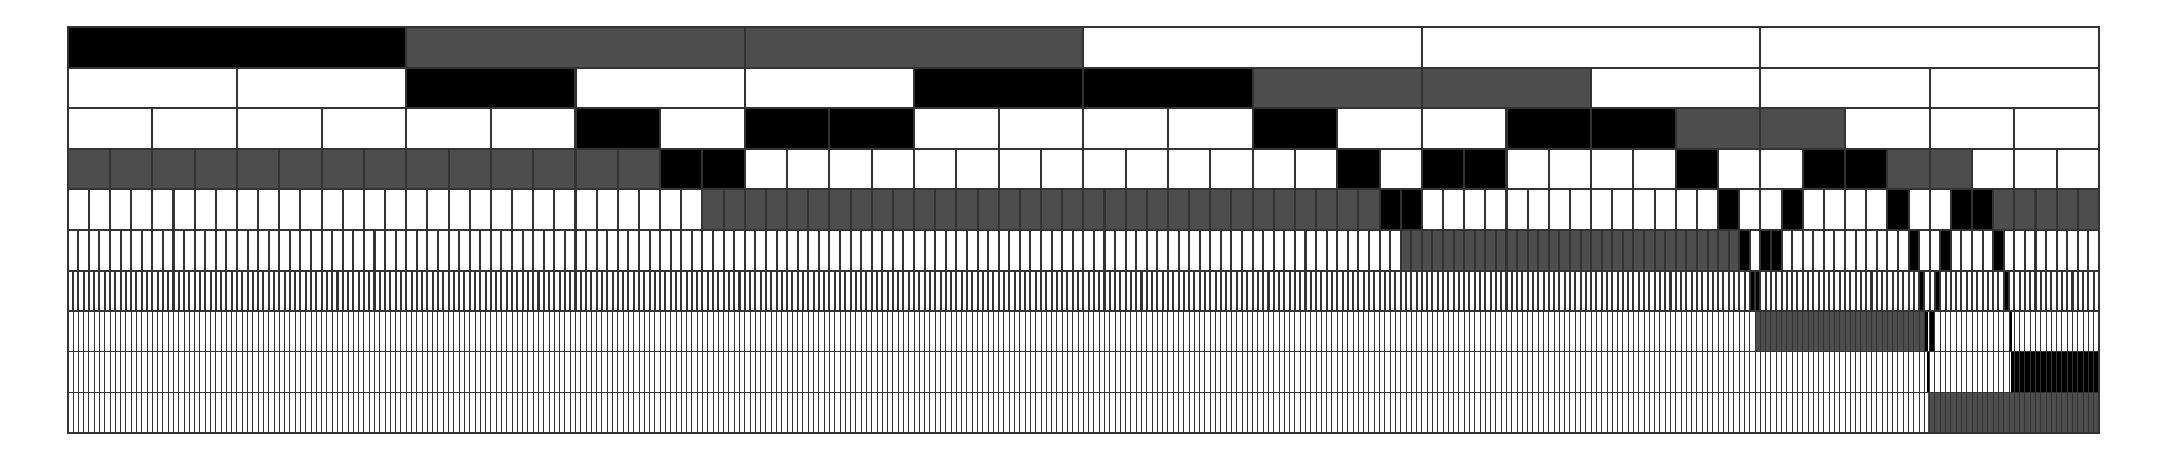
\includegraphics{2008-sica-evolution.eps}}
\caption{\label{fig:evolution} Space-time diagram of the computation of $A_M$ on input $01$.}
\end{center}
\end{figure}

We split the proof that $A_M$ is a hypercomputer into several steps.
We first show that the block transformations are well-defined and the pulse is preserved during evolution.
Afterwards we will prove that $A_M$ simulates $M$ correctly and we will show that $A_M$ represents an accelerating TM.

A configuration of the RCA $A_M$ is called finite if only a finite number of cells is different from the
quiescent state $\Box$.
Let $C$ be a finite configuration and $C^\prime$ the next configuration in the evolution of $A_M$ that is
different to $C$.
$C^\prime$ is again finite.
We denote this relationship by $C \vdash_{A_M} C^\prime$.
The relation $\vdash_{A_M}^*$ is again the reflexive and transitive closure of $\vdash_{A_M}$.
A RCA as an SCA can by definition not halt and runs forever without stopping.
The closest analogue to the TM halting occurs, when the configuration stays constant during evolution.
Such a configuration that does not change anymore is called final.

Let $D = \{\vec{\lhd}, \rhd_B, \rhd_\blacktriangleleft, \overrightarrow{a}, \overrightarrow{\langle q,a \rangle} \}$ be the
set of elements that represent the downgoing pulse,  $U = \{\blacktriangleleft\}$ be the singleton that contains the upgoing pulse,
$P = D \cup U$, and
$R = Z \backslash P$ the remaining elements.
The following lemma states the block transformations are unambiguous for the set of configurations we
consider and that the pulse is preserved during evolution.

\begin{lemma}
If the finite configuration $C$ contains exactly one element of $P$ then
the application of the block transformations \ref{tr:start-state} -- \ref{tr:up-lhd} is unambigious and at most
one block transformation is applicable.
If a configuration $C^\prime$ with $C \vdash_{A_M} C^\prime$ exists, then $C^\prime$ contains exactly one
element of $P$ as well.
\end{lemma}
\begin{proof}
Note that the domains of all block transformations are pairwise disjoint.
This ensures that for all pairs $z_1z_2$ in $Z \times Z$ at most one block transformation is applicable.
Block transformations \ref{tr:start-state} -- \ref{tr:new-blank} are all subsets or elements of
$(D \times R) \times (R \times D)$,
block transformation \ref{tr:reflection-right} is element of $(D \times R) \times (U \times R)$,
block transformations \ref{tr:up} and \ref{tr:up-state} are subsets of
$(R \times U) \times (U \times R)$, and finally
block transformation \ref{tr:up-lhd} is element of $(R \times U) \times (R \times D)$.
Since the domain is either a subset of $D \times R$ or $R \times U$ the block transformations
are unambigious if $C$ contains at most one element of $P$.
A configuration $C^\prime$ with $C \vdash_{A_M} C^\prime$ must be the result
of the application of exactly one block transformation.
Since each block transformation preserves the pulse, $C^\prime$ contains one pulse if and only if $C$ contains one.
\end{proof}

We introduce a mapping $\mathit{id}$ with the intention that finite configurations that are reached from the
initial configuration of $A_M$ are mapped to IDs of $M$.
Let $C$ be a finite configuration.
Then $\mathit  {id}C)$ is the string in $(\Gamma \cup Q)^{*}$ that is formed of $C$ as following:
\begin{enumerate}
\item All elements in $\{\Box, \blacktriangleleft, \lhd, \vec{\lhd}, \rhd, \rhd_B, \rhd_\blacktriangleleft\}$ are omitted.
\item All elements of the form $\overrightarrow{a}$ are replaced by $a$ and all elements of the form
$\langle q,a  \rangle$ or $\overrightarrow{\langle q,a  \rangle}$ are replaced by the two symbols $q$ and $a$.
\item All other elements of the form $a$ are added as they are.
\item Leading or trailing blanks of the resulting string are omitted.
\end{enumerate}
The following lemma states that $A_M$ correctly simulates $M$.
\begin{lemma}
Let $i_1$, $i_2$ be IDs of $M$.
If $i_1 \vdash_M^* i_2$, then there exist two finite configurations $C_1$, $C_2$ of $A_M$
such that $\mathit{id}(C_1) = i_1$, $\mathit{id}(C_2) = i_2$, and $C_1 \vdash_{A_M}^* C_2$.
Especially if the initial condition $C_0$ of $A_M$ satisfies  $\mathit{id}(C_0) = i_1$,
then there exists a finite configuration $C_2$ of $A_M$, such that $\mathit{id}(C_2) = i_2$
 and $C_0 \vdash_{A_M}^* C_2$.
\end{lemma}
\begin{proof}
If $i_1$ has the form $a_1 \ldots a_n q$ we consider without loss of generality $a_1 \ldots a_n q B$.
Therefore let $i_1 = a_1 \ldots a_{i-1} q a_i \ldots a_n$.
If $i < n$ or $i = n$ and $\delta_D(q, a_n) = L$ we choose
 $C_1 = \overrightarrow{\lhd}  a_1 \ldots a_{i-1} \langle q,a_i \rangle a_{i+1} \ldots a_n \rhd$.
 If $i = n$ and $\delta_D(q, a_n) = R$ we insert an additional blank:
 $C_1 = \overrightarrow{\lhd}  a_1 \ldots a_{n-1} \langle q,a_n \rangle  B \rhd$.
 In any case $\mathit{id}(C_1)=i_1$ holds.
We show the correctness of the simulation by calculating a complete zigzag of the pulse for the
start configuration:
$\overrightarrow{\lhd}  a_1 \ldots a_{i-1} \langle q,a_i \rangle a_{i+1} \ldots a_n \rhd$.
The number of the block transformation that is applied, is written above the derivation symbol.
We split the zigzag up into three phases.

\begin{enumerate}
\item Pulse moves down from the left delimiter to the left neighbor cell of the simulated head.

For $i > 1$ we obtain
\begin{equation}
\begin{array}{l}
\overrightarrow{\lhd}  a_1 \ldots a_{i-1} \langle q,a_i \rangle a_{i+1} \ldots a_n \rhd
\stackrel{(\ref{tr:start})}{\vdash_{A_M}}
\lhd  \overrightarrow{a_1} \ldots a_{i-1} \langle q,a_i \rangle a_{i+1} \ldots a_n \rhd
\stackrel{(\ref{tr:down})}{\vdash_{A_M}} \\
\lhd  a_1 \overrightarrow{a_2} \ldots a_{i-1} \langle q,a_i \rangle a_{i+1} \ldots a_n \rhd
\stackrel{(\ref{tr:down})}{\vdash_{A_M}} \ldots \stackrel{(\ref{tr:down})}{\vdash_{A_M}}
\lhd  a_1 \ldots \overrightarrow{a_{i-1}} \langle q,a_i \rangle a_{i+1} \ldots a_n \rhd.
\label{der:start}
\end{array}
\end{equation}

If $i = 1$ the pulse piggybacked by the left delimiter $\overrightarrow{\lhd}$ is already
in the left neighbor cell of the head and this phase is omitted.

\item Downgoing pulse passes the head.

If in the beginning of the zigzag the head was to the right of the left delimiter then
\begin{equation}
\overrightarrow{\lhd} \langle q,a_1 \rangle a_{2} \ldots a_n \rhd
\stackrel{(\ref{tr:start-state})}{\vdash_{A_M}}
\lhd \overrightarrow{\langle q,a_1 \rangle} a_{2} \ldots a_n \rhd
\end{equation}
If $\delta_D(q,a_1)=L$ no further block transformation is applicable and the configuration is final.
The case $\delta_D(q,a_1)=R$ will be handled later on.
We now continue the derivation~\ref{der:start}.
If $\delta(q,a_i) = (p, b, L)$ then
\begin{equation}
\lhd  a_1 \ldots \overrightarrow{a_{i-1}} \langle q,a_i \rangle a_{i+1} \ldots a_n \rhd
\stackrel{(\ref{tr:left-1})}{\vdash_{A_M}}
\lhd  a_1 \ldots \langle p,a_{i-1} \rangle \overrightarrow{b}  a_{i+1} \ldots a_n \rhd.
\label{der:tm-step-left}
\end{equation}

If $\delta(q,a_i) = (p, b, R)$ then
\begin{equation}
\lhd  a_1 \ldots \overrightarrow{a_{i-1}} \langle q,a_i \rangle a_{i+1} \ldots a_n \rhd
\stackrel{(\ref{tr:down-to-head})}{\vdash_{A_M}}
\lhd  a_1 \ldots a_{i-1} \overrightarrow{\langle q,a_i \rangle} a_{i+1} \ldots a_n \rhd.
\end{equation}
We distinguish two cases: $i < n$ and $i = n$.
If $i < n$ then
\begin{equation}
\lhd  a_1 \ldots a_{i-1} \overrightarrow{\langle q,a_i \rangle} a_{i+1} \ldots a_n \rhd
\stackrel{(\ref{tr:right-2})}{\vdash_{A_M}}
\lhd  a_1 \ldots a_{i-1} b \overrightarrow{\langle p,a_{i+1} \rangle} a_{i+2} \ldots a_n \rhd.
\label{pulse-passed}
\end{equation}
If the next steps of $M$ are moving the head again to the right, block transformation
\ref{tr:right-2} will repeatedly applied, till the head changes its direction or till the
head is left of the right delimiter $\rhd$.
If the TM $M$ changes its direction before the right delimiter is reached, we obtain
\begin{equation}
\lhd  a_1 \ldots a_{i-1} b_1 \ldots b_j \overrightarrow{\langle r ,a_{k} \rangle} a_{k+1} \ldots a_n \rhd
\stackrel{(\ref{tr:left-no-move})}{\vdash_{A_M}}
\lhd  a_1 \ldots a_{i-1} b_1 \ldots b_j \langle r ,a_{k} \rangle \overrightarrow{a_{k+1}} \ldots a_n \rhd
\end{equation}
or if the direction change happens just before the right delimiter then
\begin{equation}
\lhd  a_1 \ldots a_{i-1} b_1 \ldots b_j \overrightarrow{\langle r ,a_{n} \rangle} \rhd
\stackrel{(\ref{tr:down-state-right-delimiter})}{\vdash_{A_M}}
\lhd  a_1 \ldots a_{i-1} b_1 \ldots b_j \langle r ,a_{n} \rangle \rhd_\blacktriangleleft.
\label{der:right}
\end{equation}
If $i=n$ or if the right-moving head hits the right delimiter the derivation has the following form
\begin{equation}
\lhd  a_1 \ldots a_{n-1} \overrightarrow{\langle q,a_n \rangle}  \rhd
\stackrel{(\ref{tr:down-state-right-delimiter-blank})}{\vdash_{A_M}}
\lhd  a_1 \ldots a_{n-1} \langle q,a_n \rangle  \rhd_B
\stackrel{(\ref{tr:new-blank})}{\vdash_{A_M}}
\lhd  a_1 \ldots a_{n-1} \langle q,a_n \rangle  B \rhd_\blacktriangleleft,
\label{der:new-blank}
\end{equation}
which inserts a blank to the right of the simulated head.


\item Downgoing pulse is reflected and moves up.

We proceed from configurations of the form
$\lhd  c_1 \ldots c_{i-1} \langle p,c_{i} \rangle \overrightarrow{c_{i+1}} \ldots c_n \rhd$. Then
\begin{equation}
\begin{array}{l}
\lhd  c_1 \ldots c_{i-1} \langle p,c_{i} \rangle \overrightarrow{c_{i+1}} \ldots c_n \rhd
\stackrel{(\ref{tr:down})}{\vdash_{A_M}} \ldots \stackrel{(\ref{tr:down})}{\vdash_{A_M}}
\lhd  c_1 \ldots c_{i-1} \langle p,c_{i} \rangle c_{i+1} \ldots \overrightarrow{c_n} \rhd
\stackrel{(\ref{tr:down-a-rhd})}{\vdash_{A_M}} \\
\lhd  c_1 \ldots c_{i-1} \langle p,c_{i} \rangle c_{i+1} \ldots  c_n \rhd_\blacktriangleleft
\stackrel{(\ref{tr:reflection-right})}{\vdash_{A_M}}
\lhd  c_1 \ldots c_{i-1} \langle p,c_{i} \rangle c_{i+1} \ldots  c_n \blacktriangleleft \rhd
\stackrel{(\ref{tr:up})}{\vdash_{A_M}} \ldots \stackrel{(\ref{tr:up})}{\vdash_{A_M}} \\
\lhd  c_1 \ldots c_{i-1} \langle p,c_{i} \rangle \blacktriangleleft c_{i+1} \ldots  c_n  \rhd
\stackrel{(\ref{tr:up-state})}{\vdash_{A_M}}
\lhd  c_1 \ldots c_{i-1} \blacktriangleleft \langle p,c_{i} \rangle  c_{i+1} \ldots  c_n  \rhd
\stackrel{(\ref{tr:up})}{\vdash_{A_M}} \ldots \stackrel{(\ref{tr:up})}{\vdash_{A_M}} \\
\lhd  \blacktriangleleft c_1 \ldots c_{i-1} \langle p,c_{i} \rangle  c_{i+1} \ldots  c_n  \rhd
\stackrel{(\ref{tr:up-lhd})}{\vdash_{A_M}}
\overrightarrow{\lhd}  c_1 \ldots c_{i-1} \langle p,c_{i} \rangle  c_{i+1} \ldots  c_n  \rhd,
\end{array}
\label{der:up}
\end{equation}
which finishes the zigzag.
Note that the continuation of derivations \ref{der:right} and \ref{der:new-blank} is handled by the
later part of derivation \ref{der:up}.
We also remark that the zigzag has shifted the whole configuration one cell downwards.

\end{enumerate}

All block transformations except transformations \ref{tr:right-2} and
\ref{tr:left-1} keep the $\mathit{id}$-value of the configuration unchanged.
Block transformations \ref{tr:right-2} and \ref{tr:left-1} correctly simulate
one step in the calculation of the TM $M$:
if
$C \stackrel{(\ref{tr:right-2}) or (\ref{tr:left-1})}{\vdash_{A_M}} C^\prime$, $id(C)=i$, and $id(C^\prime)=i^\prime$
then $i \vdash_M i^\prime$.
Let $C_1^\prime$ be the resulting configuration of the zigzag.
We conclude that $\mathit{id}(C_1) \vdash_M^* \mathit{id}(C_1^\prime)$ holds.
We have chosen $C_1$ in such a way that at least one step of $M$ is performed, if $M$ does not halt, either by
block transformation \ref{tr:right-2} or \ref{tr:left-1}.
If $M$ does not halt the configuration after the zigzag is again of the form
$\overrightarrow{\lhd}  a_1 \ldots a_{i-1} \langle q,a_i \rangle a_{i+1} \ldots a_n \rhd$.
The case $i = n$ and $\delta_D(q,a_n) = R$ is excluded by derivation \ref{der:new-blank},
which inserts a blank to the right of the head, if $\delta_D(q,a_n) = R$ .
This means that $C_1^\prime$ has the same form as $C_1$ and that any subsequent zigzag will  perform at
least one step of $M$ as well if $M$ does not halt.
In summary, we conclude that $A_M$ reaches after a finite number of zigzags a configuration $C_2$ such that
$\mathit{id}(C_2) = i_2$.
On the other hand, if $M$ halts, $A_M$ enters a final configuration since derivations
\ref{der:tm-step-left} or \ref{pulse-passed} are not applicable anymore
and the pulse cannot cross the simulated head.
Since we have chosen $C_0$ to be of the same form
as $C_1$ in the beginning of the proof, the addendum of the lemma regarding the initial configuration is true.
\end{proof}

Next, the time behavior of the RCA $A_M$ will be investigated.
\begin{lemma}
Let $C=\overrightarrow{\lhd}  a_1 \ldots a_{i-1} \langle q,a_i \rangle a_{i+1} \ldots a_n \rhd$
be a finite configuration of $A_M$ that starts in cell $k$.
If $M$ does not halt, the zigzag of the pulse takes 3 cycles of cell $k$ and $A_M$
is afterwards in a finite configuration
$C^\prime=\overrightarrow{\lhd}  b_1 \ldots b_{j-1} \langle p,b_j \rangle b_{j+1} \ldots b_m \rhd$
that starts in cell $k + 1$.
\end{lemma}
\begin{proof}
Without loss of generality, we assume that the finite configuration starts in cell 0.
We follow the zigzag of the pulse, thereby tracking all times,
compare with Fig.~\ref{fig:example-hyper-sca-2} and Fig.~\ref{fig:evolution}.
The pulse reaches at time 1 cell 1,
and at time $\sum_{i=0}^1 2^{-i}$ cell 2.
In general, the downgoing pulse reaches cell $r$ in time $\sum_{i=0}^{r-1} 2^{-i}$.
At time $\sum_{i=0}^{n+1} 2^{-i}$ the cell $n+2$ changes to $\rhd_\blacktriangleleft$
which marks the reversal of direction of the pulse.
The next configuration change ($\rhd_\blacktriangleleft \Box \mapsto \blacktriangleleft \rhd$)
occurs at $\sum_{i=0}^{n+1} 2^{-i} + 2^{-(n+1)} = 2$.
The pulse $\blacktriangleleft$ reaches cell $n+1$ in time $2 + 2^{-(n+1)}$ and in general
cell $r$ in time $2 + 2^{-r}$.
The final configuration change of the zigzag ($\lhd  \blacktriangleleft \mapsto \Box  \overrightarrow{\lhd}$)
that marks also the beginning of a new pulse zigzag occurs synchronously in cell 0 and cell 1 at time 3.
We remark that the overall time of the pulse zigzag remains unchanged if the
simulated head inserts a blank between the two delimiters.
\end{proof}

\begin{theorem}
\label{th-rca}
If $M$ halts on $w$ and $A_M$ is initialized with $C_0(w)$ then $A_M$ enters a final
configuration in a time less than 6 cycles of cell 0, containing the result of the calculation between the left
and right delimiter.
If $M$ does not halt, $A_M$ enters after 6 cycles of cell 0 the final configuration that consists
of an infinite string of the quiescent element: $\Box^\infty$.
\end{theorem}
\begin{proof}
$A_M$ needs 3 cycles of cell 0 to perform the first zigzag of the pulse.
After the 3 cycles the configuration is shifted one cell downwards, starting now in cell 1.
The next zigzag takes 3 cycles of cell 1 which are 3/2 cyles of cell 0, and so on.
Each zigzags performs at least one step of the TM $M$, if $M$ does not halt.
We conclude that if $M$ halts, $A$ enters a final configuration in a time less than
$\sum_{i=0}^\infty 3/2^{i} = 6$ cycles of cell 0.
If $M$ does not halt, the zigzag disappears in infinity after 6 cycles of cell 0 leaving a trail of $\Box$'s behind.
\end{proof}

If $M$ is a universal TM, we immediately obtain the following result, which proves that $A_M$ is a hypercomputer
for certain TMs $M$.
\begin{cor}
Let $M_U$ be a universal TM. Then $A_{M_U}$ solves the halting problem for TMs.
\end{cor}
\begin{proof}
Initialize $A_{M_U}$ with an encoded TM $M$ and an input word $w$.
Then $A_M$ enters a final configuration with the result of $M$ on $w$ in less than 6 cycles of cell 0 if and only if $M$ halts.
\end{proof}

In the current form of TM simulation the operator has to scan a potentially unlimited number of cells to determine whether the
$M$ has halted or not, which limits its practical value.
If $M$ has halted, we would like to propagate at least this fact back to the upper cells.
The following obvious strategy fails in a subtle way.
Add a rule to $A_M$ that whenever $\langle q, a \rangle$ has no next move, replaces it by the new symbol $H$.
Add the rules $f_S(?, ?, H) = f_A(?, ?, H) = H$ to $A_M$
that propagate $H$ upwards to cell $0$.
The propagation upwards is only possible if we change also the block transformation \ref{tr:up-lhd}  to
$\lhd  \blacktriangleleft \mapsto \Diamond  \overrightarrow{\lhd}$,
thereby introducing a new symbol $\Diamond$ that is not subject
of the short-circuit evaluation.
The last point, even if necessary, causes the strategy to fail, since if $A_M$ does not halt,
$A_M$ is after 6 cycles in the configuration $\Diamond^\infty$ that
leads to indeterministic behavior of $A_M$.
This is in so far problematic, since we can not be sure whether a state $H$ in cell $0$
is really the outcome of a halting TM or the result of indeterministic behavior.
Instead of enhancing the RCA model, we will introduce in the next section a computing model
that is computational equivalent for finite computations, but avoids indeterminism for infinite
computations.

\section{Recursive Petri nets}
\label{chap:petri}

Time plays a crucial r\^ole in the operation of an SCA or RCA.
Failing to update the states at the required times will break the correct operation of the automaton.
This is a demanding requirement, since time intervals become arbitrarily small and
state changes have to occur globally in a certain time window, otherwise neighbor cells will get from synchronization
which leads to a malfunction of the whole automaton.
In this section, an alternative model based on Petri nets but similar to SCAs will be introduced.
The alternative model neither requires a global clock nor a simultaneous state change of neighbor cells.
It has the further property that it is not subject to indeterminism.

In what follows, we give a brief introduction to Petri nets to define the terminology.
For a more comprehensive treatment we refer to the literature; e.g., to Ref.~\cite{Murata89}.
A Petri net is a directed, weighted, bipartite graph consisting of two kinds of nodes,
called places and transitions.
In graphical representation, places are drawn as circles and transitions as boxes.
The weight $w(p,t)$ is the weight of the arc from place $p$ to transition $t$,
$w(t,p)$ is the weight of the arc from transition $t$ to place $p$.
A marking assigns to place $p$ a nonnegative integer $k$, we say that $p$ is marked with
$k$ tokens.
If a place $p$ is connected with a transition $t$ by an arc that goes from $p$ to $t$,
$p$ is an input place of $t$, if the arc goes from $t$ to $p$, $p$ is an output place.
A Petri net is changed according to the following transition (firing) rule:
\begin{enumerate}
\item
A transition $t$ fires if each input place $p$ of $t$ is marked with at least
$w(p,t)$ tokens.
\item
A firing of an enabled transition $t$ removes $w(p,t)$ tokens from each input place $p$ of $t$,
and adds $w(t,p)$ tokens to each output place $p$ of $t$.
\end{enumerate}
Formally, a Petri net $N$ is a tuple $N=(P,T,F,W,M_0)$ where
$P$ is the set of places, $T$ is the set of transitions,
$F \subseteq (P \times T) \cup (T \times P)$ is the set of arcs,
$W: F \rightarrow \mathbb{N}$ is the weight function,
and $M_0: P \rightarrow \mathbb{N}$ is the initial marking.
There are many extensions to Petri nets, one of them are the class of colored Petri nets:
In a standard Petri net, tokens are indistinguishable, whereas
in a colored Petri net, every token has a value.

\begin{figure}
\begin{center}
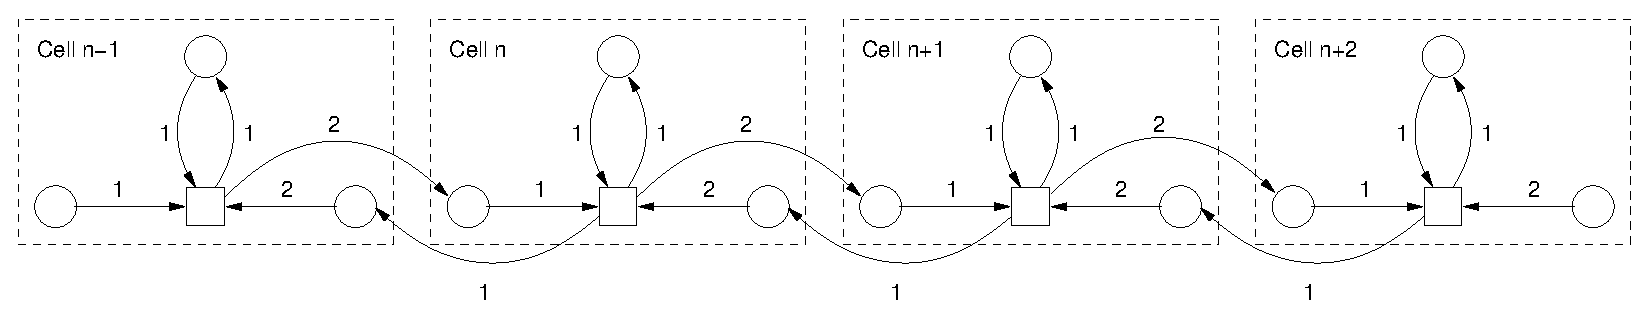
\includegraphics[scale=0.6]{2008-sica-RcaPetri.eps}
\caption{\label{petri} The underlying graph of a RPN.}
\end{center}
\end{figure}

A Recursive Petri Net (RPN) is a colored Petri net with some extensions.
The RPN  has the underlying graph partitioned into cells that is depicted in Fig.~\ref{petri}.
We denote the transition of cell $n$ by $t(n)$, the place to the left of the transition by
$p_u(n)$, the place right of the transition by $p_d(n)$ and the place above the transition by $p_c(n)$.
Let $Z$ be a finite set, the state set, $q \in Z$ be the quiescent state, and $f_A$, $f_S$ be (partial) functions $Z^4 \rightarrow Z$.
The set $V=Z \cup (\{1,2\} \times Z)$ is the value set of the tokens.
Tokens are added to a place and consumed from the place according to a first-in first-out order.
Initially, the RPN starts with a finite number of cells $0, 1, \ldots, n$, and is allowed to grow to the right.
The notation $p \leftarrow z$ defines the following action:
create a token with value $z$ and add it to place $p$.
The firing rule for a transition in cell $n$ of a RPN extends the firing rule of a standard Petri net in the following way:
\begin{enumerate}
\item If the transition $t(n)$ is enabled, the transition
removes token $\mathit{Tk}_u$ from place $p_u(n)$, token $\mathit{Tk}_c$ from $p_c(n)$ and
tokens $\mathit{Tk}_{d1}, \mathit{Tk}_{d2}$ from $p_d(n)$.
The value of token $\mathit{Tk}_{u}$ shall be of the form $(i, z_u)$ in $V=\{1,2\} \times Z$,
the other token values $z_c, z_{d1}$ and $z_{d2}$ shall be in $Z$.
If the tokens do not conform, the behavior of the transition is undefined.
\item
If $i = 1$ then let $f = f_A$ else if $i = 2$ then let $f = f_S$.
The transition calculates $z = f(z_u, z_c, z_{d1}, z_{d2})$.
\item
\emph{(Left boundary cell)}
If $n = 0$ then
$p_u(0) \leftarrow (3 - i, q)$, $p_c(0) \leftarrow z$, $p_u(1) \leftarrow (1, z)$, $p_u(1) \leftarrow (2,z)$.
\item
\emph{(Inner cell)}
If $n > 0$ and $n$ is not the highest index, then:
$p_d(n-1) \leftarrow z$, $p_c(n) \leftarrow z$, $p_u(n+1) \leftarrow (1, z)$, $p_u(n+1) \leftarrow (2, z)$.
\item \emph{(Right boundary cell)}
If $n$ is the highest index then:
\begin{enumerate}
\item \emph{(Quiescent state)}
\label{firing-rule-quiescent}
If $z = q$ then
$p_d(n-1) \leftarrow q$, $p_c(n) \leftarrow q$, $p_d(n) \leftarrow q$, $p_d(n) \leftarrow q$
\item \emph{(New cell allocation)}
If $z \neq q$ then a new cell $n + 1$ is created and connected to cell $n$.
Furthermore: $p_d(n-1) \leftarrow z$, $p_c(n) \leftarrow z$, $p_d(n) \leftarrow q$,
$p_u(n+1) \leftarrow (1, z)$, $p_u(n+1) \leftarrow (2, z)$,
$p_c(n + 1) \leftarrow q$, $p_d(n + 1) \leftarrow q$, $p_d(n + 1) \leftarrow q$.
\end{enumerate}
\end{enumerate}
Formally, we denote the RPN by a tuple $N = (Z, f_A, f_S)$.
Let $a_0 a_1 \ldots a_m$ be an input word in $Z^{m+1}$ and let
$N$ be a RPN with $n$ cells, whereby $n > m + 1$.
The initial markup of the Petri net is as follows:
\begin{itemize}
\item $p_u(0) \leftarrow (1, q)$,
($p_u(i) \leftarrow (1, a_{i-1})$, $p_u(i) \leftarrow (2, a_{i-1})$) for $0 < i \leq m + 1$,
($p_u(i) \leftarrow (1, q)$, $p_u(i) \leftarrow (2, q)$) for  $i > m + 1$
\item $p_c(i) \leftarrow a_i$ for $i \leq m$, $p_c(i) \leftarrow q$ for $i > m$,
\item
$p_d(i) \leftarrow a_{i+1}$ for $i < m$, $p_d(i) \leftarrow q$ for $i \geq m$, and $p_d(n) \leftarrow q$.
\end{itemize}
Note that the place $p_d(n)$ is initialized with two tokens.
We identify the state of a cell with the value of its $p_c$-token.
If $p_c$ is empty, because
the transition is in the process of firing, the state shall be the value of the last consumed token of $p_c$.

\begin{figure}
\begin{center}
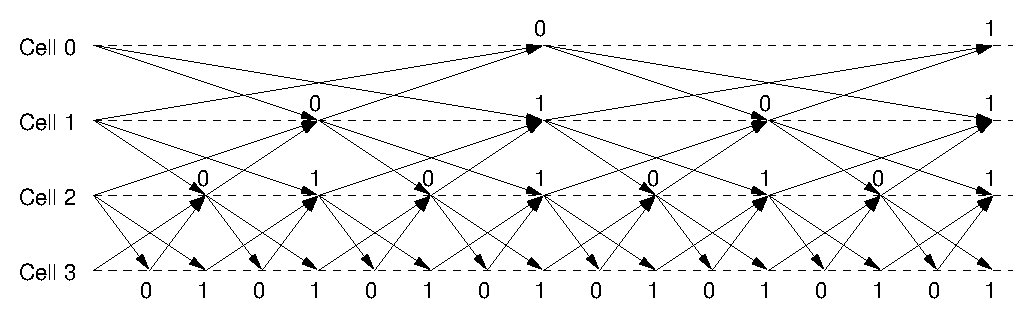
\includegraphics[scale=0.8]{2008-sica-TokenFlow.eps}
\caption{\label{token-flow} Token flow in a RPN.}
\end{center}
\end{figure}

Fig.~\ref{token-flow} depicts the token flow of a RPN net consisting of $4$ cells under the assumption
that the RPN does not grow.
Tokens that are created and consumed by the same cell are not shown.
The numbers indicate whether the firing is asynchronous (1) or synchronous (2).
The only transition that is enabled in the begin is $t(3)$, since $p_d(3)$ was initialized with 2 tokens.
The firing of $t(3)$ bootstrap the RPN by adding a second token to $p_d(2)$, thereby enabling $t(2)$, and so on,
till are transitions have fired,
and the token flow enters periodic behavior.

We now compare RPNs with RCAs.
We call a computation finite, if it involves either only a finite number of state updates of a RCA, or
a finite number of transition firings of a RPN, respectively.
\begin{lemma}
\label{lemma:comp-equivalence}
For a finite computation, a dynamically growing RCA $A = (Z, f_A, f_S)$ and a RPN $N = (Z, f_A, f_S)$ are computationally
equivalent on a step-by-step basis if the start with the same number of cells and the same initial configuration.
\end{lemma}
\begin{proof}
Let $N$ be a RPN that has initially $n$ cells.
For the purpose of the proof consider an enhanced RPN $N^\prime$ that is able to timestamp its token.
A token $\mathit{Tk}$ of $N^\prime$ does not hold only a value, but also a time interval.
We refer to the time interval of $\mathit{Tk}$ by $\mathit{Tk}.t$ and to the value of $\mathit{Tk}$ by $\mathit{Tk}.v$.
We remark that the timestamps serve only to compare the computations of a RCA and a RPN and do not imply any time behaviour of the RPN.
The firing rule of $N^\prime$ works as for $N$, but has an additional pre- and postprocessing step:
\begin{itemize}
\item \emph{(Preprocessing)}
Let $\mathit{Tk}_c$, $\mathit{Tk}_u$, $\mathit{Tk}_{d1}$, and $\mathit{Tk}_{d2}$ be the consumed token, where the alphabetical subscript denotes
the input place and the numerical subscript the order in which the tokens were consumed.
Calculate $t = (\mathit{Tk}_c.t)_\rightarrow$, where $\rightarrow$ is the inverse time operator of $\leftarrow$.
If $\mathit{Tk}_{d1}.t \neq t_\swarrow$ or $\mathit{Tk}_{d2}.t \neq t_\searrow$ or $\mathit{Tk}_{u}.t \neq t_\uparrow$ the firing fails
and the transition becomes permanently disabled.
\item \emph{(Postprocessing)}
For each created token $\mathit{Tk}$, set $\mathit{Tk}.t = t$.
\end{itemize}
The initial marking must set the $t$-field, otherwise the first transitions will fail.
For the initial tokens in cell $k$,
set $\mathit{Tk}_u.t = 2^{-k+1} \mathbbm{1}$ for both tokens in place $p_u$, $\mathit{Tk}_c.t = 2^{-k} \mathbbm{1}$,
and $\mathit{Tk}_d.t = 2^{-k-1} \mathbbm{1}$.
Set $\mathit{Tk}_d.t = 2^{-n-1} (1 + \mathbbm{1})$ for the second token in $p_d(n)$.
The firings of cell $k$ add tokens with timestamps $2^{-k} \mathbbm{1}, 2^{-k} (2 + \mathbbm{1}), 2^{-k} (3 + \mathbbm{1}) \ldots$
to the output place $p_c(k)$.
If transition $t(k)$ does not fail, the state function for the arguments $c=2^{-k} \mathbbm{1}$ and $t=2^{-k} (i + \mathbbm{1})$ is well-defined:
$s^\prime(c,t) = z$ if cell $k$ has produced or was initialized in place $p_d$ with a token $\mathit{Tk}$ with $\mathit{Tk}.t = t$ and $\mathit{Tk}.v = z$.
Let $s(c,t)$ be the state function of the SCA $A$.
Due to the initialization, the two state functions are defined for the first $n$ cells and first time intervals $2^{-k} \mathbbm{1}$.
Assume that the values of $s$ and $s^\prime$ differ for some argument or that their domains are different.
Consider the first time interval $t_1$ where the difference occurs:
$s(c,t_1) \neq s^\prime(c,t_1)$, or exactly one of $s(c,t_1)$ or $s^\prime(c,t_1)$ is undefined.
If there is more than one time interval choose an arbitrary one of these.
Since $t_1$ was the first time interval where the state functions differ, we know that
$s(c_\uparrow, {t_1}_\uparrow) = s^\prime(c_\uparrow, {t_1}_\uparrow)$,
$s(c, {t_1}_\leftarrow) = s^\prime(c, {t_1}_\leftarrow)$,
$s(c_\swarrow, {t_1}_\swarrow) = s^\prime(c_\swarrow, {t_1}_\swarrow)$, and
$s(c_\swarrow, {t_1}_\searrow)= s^\prime(c_\swarrow, {t_1}_\searrow)$.
We handle the case that the values of the state functions are different or that $s^\prime$ is undefined for $(c,t_1)$ whereas $s$ is.
The other case ($s^\prime$ defined, but not $s$) can be handled analogously.
If $c = 2^{-k} \mathbbm{1}$, we conclude that tokens with timestamps ${t_1}_\uparrow$, ${t_1}_\leftarrow$, ${t_1}_\swarrow$, ${t_1}_\searrow$ were sent
to cell $k$, and no other tokens were sent afterwards to cell $k$, since the timestamps are created in
chronological order.
Hence, the precondition of the firing rule is satisfied and we conclude that $s(c,t_1) = s^\prime(c,t_1)$, which contradicts our assumption.
The allocation of new cells introduces some technicalities, but the overall strategy of going back in time
and concluding that the conditions for a state change or cell allocation were the same in both models works here also.
We complete the proof, by the simple observation that $N$ and $N^\prime$ perform the same computation.
\end{proof}
The proof can be simplified using the following more abstract argumentation.
A comparison of Fig.~\ref{token-flow} with Fig.~\ref{fig:timeops} shows that each computation step has in both models
the same causal dependencies.
Since both computers use the same rule to calculate the value of a cell, respectively the value of a token,
we conclude that the causal nets \cite{Levin81} of both computations are the same for a finite computation,
and therefore both computers yield the same output, in case the computation is finite.

Till now, the RPN model is purely computational.
We use the following mapping to space-time.
The length of cell $k$ is $2^{-k}$ and the cells are arranged as the cells of a RCA .
Under the assumption of a constant token speed, a firing time that is  proportional to the cell length,
and an appropriate unit of time
we yield  again cycle times of $2^{-k}$.

We now come back to the simulation of TMs and construct a hypercomputing RPN, analogous to the
hypercomputing RCA in section \ref{chap:hypercomputer}.
Let $M = (Q, \Sigma, \Gamma, \delta, q_0, B, F)$ be an arbitrary TM.
Let $Z$ be the state set that we used in the simulation of a TM by a RCA, and let
$f_A$, $f_S$ the functions that are defined by the block transformations \ref{tr:start-state} - \ref{tr:up-lhd},
without the short-circuit evaluation.
By Lemma \ref{lemma:comp-equivalence} we know that the RPN $N_M = (Z, f_A, f_S)$ simulates $M$ correctly for a finite number of TM steps.
Hence, if $M$ halts on input $w$, $N_M$ enters a final configuration in less than 6 cyles of cell 0.
We examine now the case that $M$ does not halt.
A pivotal difference between a RCA and a RPN is the ability of the latter one to halt on a computation.
This happens if all transitions of the RPN are disabled.

\begin{lemma}
\label{lemma:apn-halting}
Let $M = (Q, \Sigma, \Gamma, \delta, q_0, B, F)$ be an arbitrary TM and $w$ an input word in $\Sigma^*$.
If $M$ does not halt on $w$, the RPN $N_M$ halts on $C_0(w)$ after 6 cycles of cell 0.
\end{lemma}
\begin{proof}
As long as the number of cells is finite, the boundary condition~\ref{firing-rule-quiescent} of the firing rule adds by each firing
two tokens to the $p_d$-place of the rightmost cell that successively enable all other transitions as well.
This holds no longer for the infinite case.
Let $M$ be a TM, and $w$ an input word, such that $M$ does not halt on $w$.
We consider again the travel of the pulse zigzags down to infinity for the RPN $N_M$ with
initial configuration $C_0(w)$, thereby tracking the marking of the $p_d$-places
for times after the zigzag has passed by.
The first states of cell $0$ are $\overrightarrow{\lhd}$, $\lhd$, $\lhd$, and $\Box$, including the initial one.
The state $\Box$ is the result of the firing at time 3, exhausting thereby the tokens in place $p_d(0)$.
At time 3 the left delimiter ($\overrightarrow{\lhd}$) of the pulse zigzag is now in cell 1.
Cell 1 runs from time 3 on through the same state sequence $\overrightarrow{\lhd}$, $\lhd$, $\lhd$, and $\Box$,
thereby adding in summary 4 tokens to $p_d(0)$.
After creating the token with value $\Box$, $p_d(1)$ is empty as well.
We conclude that after the zigzag has passed by a cell, the lower cell sends in summary 4 tokens to the upper cell,
till the zigzag has left the lower cell as well.
For each cell $k$ these four tokens in $p_d(k)$ enable two firings of cell $k$ thereby adding two tokens
to $p_d(k-1)$.
These two tokens of $p_d(k-1)$ enable again one firing of cell $k-1$ thereby adding one token to $p_d(k-2)$.
We conclude that each cell fires 3 times after the zigzag has passed by and that the final marking of each $p_d$ is one.
Hence, no $p_d$ has the necessary two tokens that enable the transition, therefore all transitions are disabled
and $N_M$ halts at time 6.
\end{proof}

Since $N_M$ halts for nonhalting TMs, there are no longer any obstacles that prevent
the construction of the proposed propagation of the halting state back to upper cells.
We replace block transformation \ref{tr:start-state} with the following two and add one new.

If $\delta(q,a) = (p,c,R)$ set
\begin{equation}
\overrightarrow{\lhd} \: \langle q, a \rangle \mapsto \lhd \:
\overrightarrow{\langle q, a \rangle}.
\label{tr:start-state2}
\end{equation}

If $\delta(q,a) = (p,c,L)$ or $\delta(q,a)$ is not defined set
\begin{equation}
\overrightarrow{\lhd} \: \langle q, a \rangle \mapsto \lhd \: H.
\label{tr:H}
\end{equation}

If $\delta(q,a)$ is not defined set
\begin{equation}
\overrightarrow{b} \: \langle q, a \rangle \mapsto b \: H.
\label{tr:down-to-head2}
\end{equation}

The following definition propagates the state $H$ up to cell $0$:
\begin{equation}
f_A(?, ?, H) = f_S(?, ?, H) = H.
\label{eq:H-up}
\end{equation}
We denote the resulting RPN by $\overline{N}_M$.
The following theorem makes use of the apparently paradoxical fact, that $\overline{N}_M$ halts if and only if the
simulated TM does not halt.
\begin{theorem}
Let $M_U$ be a universal TM. Then $\overline{N}_{M_U}$ solves the halting problem for TMs.
\end{theorem}
\begin{proof}
Consider a TM $M$ and an input word $w$. Initialize $\overline{N}_{M_U}$ with $C_0(\langle M, w \rangle )$ where
$\langle M, w \rangle$ is the encoding of $M$ and $w$.
If $M$ does not halt on $w$, $\overline{N}_{M_U}$ halts at time 6 by Lemma~\ref{lemma:apn-halting}.
If $M$ halts on $w$, then one cell of $\overline{N}_{M_U}$ enters the state $H$ by
block transformation~\ref{tr:H} or~\ref{tr:down-to-head2} according to
Theorem~\ref{th-rca} and Lemma~\ref{lemma:comp-equivalence} and taking the changes in $f_A$ and $f_S$ into account.
The mapping~\ref{eq:H-up} propagates $H$ up to cell 0.
An easy calculation shows that cell 0 is in state $H$, in time 7 or less.
\end{proof}

We have proven that $\overline{N}_{M_U}$ is indeed a hypercomputer without the deficiencies of the SCA-based
hypercomputer. We end this section with two remarks.
The RPN $N_M$ sends a flag back to the upper cells, if the simulated TM halts.
Strictly speaking, this is not necessary, if the operator is able to recognize whether the RPN has halted or not.
On the other hand, a similar construction is essential, if the operator is interested in the final tape content of the
simulated TM.
Transferring the whole tape content of the simulated TM upwards,
could be achieved by implementing a second pulse that performs an upwards-moving zigzag.
The construction is even simpler as the described one, since the tape content of the TM becomes static, as soon as the TM halts.
The halting problem of TMs is not the only problem that can be solved by RCAs or SCAs, but is unsolvable for TMs.
A discussion of other problems unsolvable by TMs and of techniques to solve them within infinite computing machines, can be found in
Davies~\cite{Davies01}.

\section{Summary}

We have presented two new computing models that implement the potential
infinite divisibility of physical configuration space.
These models are purely information theoretic and
do not take into account kinetic and other
effects.
With these provisos, it is possible, at least in
principle, to use the potential infinite
divisibility of space-time to perform hypercomputation,
thereby extending the algorithmic domain to hitherto unsolvable decision problems.

Both models are composed of elementary computation primitives.
The two models are closely related but are very different ontologically.
A cellular automaton depends on an {\em extrinsic} time requiring an {\em external} clock
and a rigid synchronization of its computing cells, whereas
a Petri net implements a causal relationship leading to an {\em intrinsic} concept of time.

SCAs as well as RPNs are built the same way from their primitive building blocks.
Each unit is recursively coupled with a sized-down copy of itself, potentially leading
to an infinite sequence of ever decreasing units.
Their close resemblance leads to a step-by-step equivalence of finite computations,
yet their ontological difference yields different behavior for the infinite case:
an SCA exhibits indeterministic behavior, whereas a RPN halts.
Two supertasks which operate identically in the finite case but differ in
their limit is a puzzling observation which might question our hitherto understanding of supertasks.
This may be considered an analogy to a theorem \cite{Specker49} in recursive analysis
about the existence of recursive monotone bounded sequences of rational numbers
whose limit is not a computable number.

One striking feature of both models is their scale-invariance.
The computational behavior of these models is therefore the first example for what might be called
scale-invariant computing, which might be characterized by the property that
any computational space-time pattern can be arbitrary squeezed to finer and finer regions of space and time.

Although the basic definitions have been given, and elementary properties of these new models have been explored,
a great number of questions remain open for future research.
The construction of a hypercomputer was a first demonstration of the
extraordinary computational capabilities of these models.
Further investigations are necessary to determine their limits, and to relate them with the
emerging field of hypercomputation~\cite{2002-cal-pav,ord-2002,Davis-2004,Doria-2006,Davis-2006}.
Another line of research would be the investigation of their phenomenological properties, analogous
to the statistical mechanics of cellular automata~\cite{wolfram83,wolfram-2002}.

%\bibliography{svozil}
%\bibliographystyle{osa}


\begin{thebibliography}{10}
\newcommand{\enquote}[1]{``#1''}
\expandafter\ifx\csname url\endcsname\relax
  \def\url#1{{#1}}\fi
\expandafter\ifx\csname urlprefix\endcsname\relax\def\urlprefix{}\fi

\bibitem{landauer-89}
R.~Landauer, \enquote{Computation, Measurement, Communication and Energy
  Dissipation,} in {\em Selected Topics in Signal Processing\/}, S.~Haykin, ed.
   (Prentice Hall, Englewood Cliffs, NJ, 1989), p.~18.

\bibitem{maxwell-demon}
H.~S. Leff and A.~F. Rex, {\em Maxwell's Demon\/} (Princeton University Press,
  Princeton, 1990).

\bibitem{bennett-73}
C.~H. Bennett, \enquote{Logical Reversibility of Computation,} IBM Journal of
  Research and Development {\bf 17}, 525--532 (1973), reprinted in \cite[pp.
  197-204]{maxwell-demon}.

\bibitem{v-neumann-66}
J.~von Neumann, {\em Theory of Self-Reproducing Automata\/} (University of
  Illinois Press, Urbana, 1966), a. W. Burks, editor.

\bibitem{zuse-67}
K.~Zuse, \enquote{{R}echnender {R}aum,} Elektronische Datenverarbeitung pp.
  336--344 (1967).
\newline http://www.idsia.ch/~juergen/digitalphysics.html

\bibitem{zuse-69}
K.~Zuse, {\em {R}echnender {R}aum\/} (Friedrich Vieweg \& Sohn, Braunschweig,
  1969), {E}nglish translation \cite{zuse-70}.

\bibitem{zuse-94}
K.~Zuse, \enquote{Discrete Mathematics and {R}echnender {R}aum,}  (1994).
\newline http://www.zib.de/PaperWeb/abstracts/TR-94-10/

\bibitem{zuse-70}
K.~Zuse, {\em Calculating Space. MIT Technical Translation AZT-70-164-GEMIT\/}
  (MIT (Proj. MAC), Cambridge, MA, 1970).

\bibitem{fredkin}
E.~Fredkin, \enquote{An informational process based on reversible universal
  cellular automata,} Physica {\bf D45}, 254--270 (1990).
\newline http://dx.doi.org/10.1016/0167-2789(90)90186-S

\bibitem{toffoli-margolus-90}
T.~Toffoli and N.~Margolus, \enquote{Invertible cellular automata: A review,}
  Physica D {\bf 45}, 229--253 (1990).
\newline http://dx.doi.org/10.1016/0167-2789(90)90185-R

\bibitem{wolfram-2002}
S.~Wolfram, {\em A New Kind of Science\/} (Wolfram Media, Inc., Champaign, IL,
  2002).

\bibitem{hopcroft}
J.~E. Hopcroft and J.~D. Ullman, {\em Introduction to Automata Theory,
  Languages, and Computation\/} (Addison-Wesley, Reading, MA, 1979).

\bibitem{svozil-94}
K.~Svozil, \enquote{Extrinsic-intrinsec concept and complementarity,} in {\em
  Inside versus Outside\/}, H.~Atmanspacker and G.~J. Dalenoort, eds.
  (Springer-Verlag, Heidelberg, 1994), pp. 273--288.

\bibitem{toffoli:79}
T.~Toffoli, \enquote{The role of the observer in uniform systems,} in {\em
  Applied General Systems Research, Recent Developments and Trends\/}, G.~J.
  Klir, ed.  (Plenum Press, New York, London, 1978), pp. 395--400.

\bibitem{zeno}
H.~D.~P. Lee, {\em Zeno of Elea\/} (Cambridge University Press, Cambridge,
  1936), reprinted by Adolf M. Hakkert, Amsterdam, 1967.

\bibitem{ki-57}
G.~S. Kirk and J.~E. Raven, {\em The Presocratic Philosophers\/} (Cambridge
  University Press, Cambridge, 1957).

\bibitem{gruenbaum:68}
A.~Gr{\"{u}}nbaum, {\em Modern Science and Zeno's paradoxes\/} (Allen and
  Unwin, London, 1968), second edition edn.

\bibitem{sv-aut-rev}
K.~Svozil, \enquote{The {C}hurch-{T}uring Thesis as a Guiding Principle for
  Physics,} in {\em Unconventional Models of Computation\/}, C.~S. Calude,
  J.~Casti, and M.~J. Dinneen, eds.,  pp. 371--385 (1998).
\newline http://arxiv.org/abs/quant-ph/9710052

\bibitem{weyl:49}
H.~Weyl, {\em Philosophy of Mathematics and Natural Science\/} (Princeton
  University Press, Princeton, 1949).

\bibitem{Davies01}
E.~B. Davies, \enquote{Building Infinite Machines,} The British Journal for the
  Philosophy of Science {\bf 52}, 671--682 (2001).
\newline http://dx.doi.org/10.1093/bjps/52.4.671

\bibitem{gruenbaum:74}
A.~Gr{\"{u}}nbaum, {\em Philosophical problems of space and time (Boston
  Studies in the Philosophy of Science, vol. 12)\/} (D. Reidel,
  Dordrecht/Boston, 1974), second, enlarged edition edn.

\bibitem{svozil98}
K.~Svozil, \enquote{The {C}hurch-{T}uring Thesis as a Guiding Principle for
  Physics,} in {\em Unconventional Models of Computation\/}, C.~S. Calude,
  J.~Casti, and M.~J. Dinneen, eds.,  pp. 371--385 (1998).
\newline http://arxiv.org/abs/quant-ph/9710052

\bibitem{rucker}
R.~Rucker, {\em Infinity and the Mind\/} (Birkh{\"{a}}user, Boston, 1982),
  reprinted by Bantam Books, 1986.

\bibitem{ord-2006}
T.~Ord, \enquote{The many forms of hypercomputation,} Applied Mathematics and
  Computation {\bf 178}, 143--153 (2006).
\newline http://dx.doi.org/10.1016/j.amc.2005.09.076

\bibitem{Davis-2004}
M.~Davis, \enquote{The myth of hypercomputation,} in {\em Alan Turing: Life and
  Legacy of a Great Thinker\/}, C.~Teuscher, ed.  (Springer, Berlin, 2004), pp.
  195--212.

\bibitem{Doria-2006}
F.~A. Doria and J.~F. Costa, \enquote{Introduction to the special issue on
  hypercomputation,} Applied Mathematics and Computation {\bf 178}, 1--3
  (2006).
\newline http://dx.doi.org/10.1016/j.amc.2005.09.065

\bibitem{Davis-2006}
M.~Davis, \enquote{Why there is no such discipline as hypercomputation,}
  Applied Mathematics and Computation {\bf 178}, 4--7 (2006).
\newline http://dx.doi.org/10.1016/j.amc.2005.09.066

\bibitem{thom:54}
J.~F. Thomson, \enquote{Tasks and supertasks,} Analysis {\bf 15}, 1--13 (1954).

\bibitem{benna:62}
P.~Benacerraf, \enquote{Tasks and supertasks, and the modern {E}leatics,}
  Journal of Philosophy {\bf LIX}, 765--784 (1962).

\bibitem{pit:90}
I.~Pitowsky, \enquote{The physical {C}hurch-{T}uring thesis and physical
  computational complexity,} Iyyun {\bf 39}, 81--99 (1990).

\bibitem{ear-nor:93}
J.~Earman and J.~D. Norton, \enquote{Forever is a day: supertasks in {P}itowsky
  and {M}alament-{H}ogart spacetimes,} Philosophy of Science {\bf 60}, 22--42
  (1993).

\bibitem{hogarth1}
M.~Hogarth, \enquote{Predicting the future in relativistic spacetimes,} Studies
  in History and Philosophy of Science. Studies in History and Philosophy of
  Modern Physics {\bf 24}, 721--739 (1993).

\bibitem{hogarth2}
M.~Hogarth, \enquote{Non-{T}uring computers and non-{T}uring computability,}
  PSA {\bf 1}, 126--138 (1994).

\bibitem{beth-59}
E.~W. Beth, {\em The Foundations of Metamathematics\/} (North-Holland,
  Amsterdam, 1959).

\bibitem{le-91}
E.~G.~K. L{\'{o}}pez-Escobar, \enquote{{Z}eno's Paradoxes: Pre {G}{\"{o}}delian
  Incompleteness,} Yearbook 1991 of the Kurt-G{\"{o}}del-Society {\bf 4},
  49--63 (1991).

\bibitem{wolfram-86}
S.~Wolfram, {\em Theory and Application of Cellular Automata\/} (World
  Scientific, Singapore, 1986).

\bibitem{gutowitz}
H.~Gutowitz, \enquote{Cellular Automata: Theory and Experiment,} Physica {\bf
  D45}, 3--483 (1990), previous CA conference proceedings in {\em International
  Journal of Theoretical Physics} {\bf 21}, 1982; as well as in {\em Physica},
  {\bf D10}, 1984 and in {\bf Complex Systems} {\bf 2}, 1988.

\bibitem{ilachinski01}
A.~Ilachinski, {\em Cellular Automata: A Discrete Universe\/} (World Scientific
  Publishing Co., Inc., River Edge, NJ, USA, 2001).

\bibitem{Morelli_Zanette}
L.~G. Morelli and D.~H. Zanette, \enquote{Synchronization of stochastically
  coupled cellular automata,} Physical Review E {\bf 58}, R8--R11 (1998).
\newline http://dx.doi.org/10.1103/PhysRevE.58.R8

\bibitem{BoFeng_MengDing}
B.~Feng and M.~Ding, \enquote{Block-analyzing method in cellular automata,}
  Physical Review E {\bf 52}, 3566--3569 (1995).
\newline http://dx.doi.org/10.1103/PhysRevE.52.3566

\bibitem{Brunnet_Chate}
L.~G. Brunnet and H.~Chat{\'{e}}, \enquote{Cellular automata on
  high-dimensional hypercubes,} Physical Review E {\bf 69}, 057\,201 (2004).
\newline http://dx.doi.org/10.1103/PhysRevE.69.057201

\bibitem{Murata89}
T.~Murata, \enquote{Petri nets: Properties, analysis and applications,}
  Proceedings of the IEEE {\bf 77}, 541--580 (1989).
\newline http://dx.doi.org/10.1109/5.24143

\bibitem{Levin81}
L.~A. Levin, \enquote{Causal Nets or What is a Deterministic Computation,}
  Information and Control {\bf 51}, 1--19 (1981).

\bibitem{Specker49}
E.~Specker, \enquote{Nicht konstruktiv beweisbare {S}\"atze der {A}nalysis,}
  The Journal of Smbolic Logic {\bf 14}, 145--158 (1949), reprinted in
  \cite[pp. 35--48]{specker-ges}; {E}nglish translation: {\it Theorems of
  Analysis which cannot be proven constructively}.

\bibitem{2002-cal-pav}
C.~S. Calude and B.~Pavlov, \enquote{Coins, Quantum Measurements, and
  {T}uring's Barrier,} Quantum Information Processing {\bf 1}, 107--127 (2002).
\newline http://arxiv.org/abs/quant-ph/0112087

\bibitem{ord-2002}
T.~Ord, \enquote{Hypercomputation: computing more than the Turing machine,}
  (2002).
\newline http://arxiv.org/abs/math/0209332

\bibitem{wolfram83}
S.~Wolfram, \enquote{Statistical Mechanics of Cellular Automata,} Reviews of
  Modern Physics {\bf 55}, 601--644 (1983).

\bibitem{specker-ges}
E.~Specker, {\em Selecta\/} (Birkh{\"{a}}user Verlag, Basel, 1990).

\end{thebibliography}
\end{document}
